%%%%%%%%%%%%%%%%%%%%%%%%%%%%%%%
% COM2005-3005 Bio-Inspired Computing and Robotics
% Robotics Lab Assignment Report Template
% Prof. Roger K. Moore
% University of Sheffield
% 10 April 2018
%%%%%%%%%%%%%%%%%%%%%%%%%%%%%%%

\documentclass[hidelinks,a4paper,11pt]{article}

\usepackage[margin=1.2in]{geometry}
\usepackage{graphicx}
\usepackage{array}
\usepackage{hyperref}
\usepackage[parfill]{parskip}
\usepackage{mdframed}
\usepackage{enumitem,amssymb}
\usepackage{gensymb}
\usepackage{siunitx}
\newlist{todolist}{itemize}{2}
\setlist[todolist]{label=$\square$}
\usepackage{pifont}
\newcommand{\cmark}{\ding{51}}%
\newcommand{\xmark}{\ding{55}}%
\newcommand{\done}{\rlap{$\square$}{\raisebox{2pt}{\large\hspace{1pt}\cmark}}
\hspace{-2.5pt}}
\newcounter{question}
\newcommand\myq{\refstepcounter{question}\thequestion}
\newcolumntype{P}[1]{>{\centering\arraybackslash}p{#1}}
\usepackage{gensymb}


\begin{document}

\begin{titlepage}

\begin{center}
{\LARGE University of Sheffield}\\[1cm]
\huge {\bfseries COM2005-3005\\Bio-inspired Computing and Robotics}\\[1cm]

\includegraphics[width=5cm]{tuoslogo.png}\\[1cm]
{\LARGE Robotics Lab Assignment}\\[2cm]

%vvvvvvvvvvvvvvvvvvvvvvvvvvvvvvvvvvvvvvvvvvvvvvvvvvvvvvvvvvvvvv
% DELETE (OR COMMENT OUT) THESE TWO LINES
% {\huge \bfseries Instructions}\\[0.5cm]
% {\Large Prof. Roger K. Moore}\\[1cm]
%^^^^^^^^^^^^^^^^^^^^^^^^^^^^^^^^^^^^^^^^^^^^^^^^^^^^^^^^^^^^^^^^^^

%vvvvvvvvvvvvvvvvvvvvvvvvvvvvvvvvvvvvvvvvvvvvvvvvvvvvvvvvvvvvvv
% EDIT YOUR NAMES (AND UNCOMMENT)
{\Large Catalin	Mares}\\
{\Large David Coelho}\\
{\Large Huzaifa	Ahmed}\\
{\Large Joseph Slade}\\
{\Large Zer Jun Eng}\\[1cm]
%^^^^^^^^^^^^^^^^^^^^^^^^^^^^^^^^^^^^^^^^^^^^^^^^^^^^^^^^^^^^^^^^^^

%vvvvvvvvvvvvvvvvvvvvvvvvvvvvvvvvvvvvvvvvvvvvvvvvvvvvvvvvvvvvvv
% EDIT THE ID OF YOUR ROBOT (AND UNCOMMENT)
{\LARGE Robot: A2}\\[1cm]
%^^^^^^^^^^^^^^^^^^^^^^^^^^^^^^^^^^^^^^^^^^^^^^^^^^^^^^^^^^^^^^^^^^

{\LARGE Department of Computer Science}\\
{\Large \today}
\end{center}

\end{titlepage}

\tableofcontents
\newpage


\section{Part I: Experiments with a PID Controller}

\subsection{General Principles}

Recall from Prof.\ Moore's Lecture-2 on `Autonomous Systems' that a classic negative-feedback
control system is structured as follows:\\
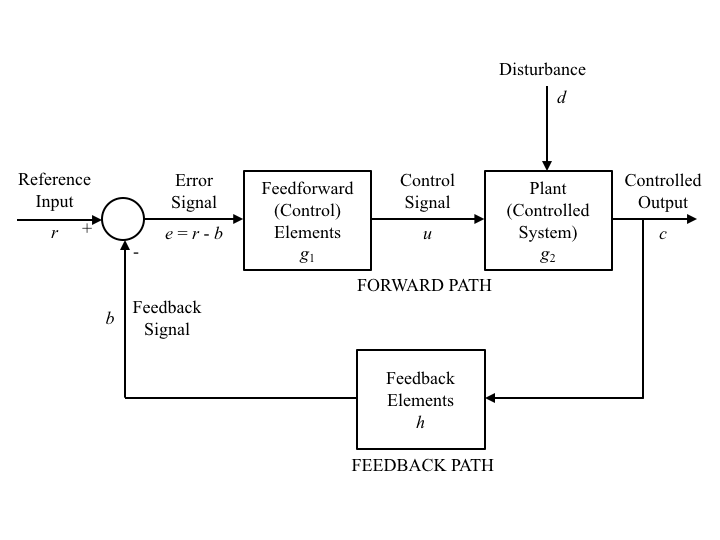
\includegraphics[width=\textwidth]{ClassicControlSystem.png}
Recall also that $g_1$ is commonly configured as a proportional-integral-derivative (PID)
controller.  Mathematically, this takes the form:
$$u(t) = K_P e(t) + K_I \int e(t)dt + K_D \frac{de}{dt}(t) ,$$ \ldots where $K{_P}$ is the
proportional gain, $K_I$ is the integral gain and $K_D$ is the derivative gain.  A simple
proportional controller would use $K_P$ only (i.e.\ $K_I=0$ and $K_D=0$).

In order to ensure that you fully understand these basic principles, please provide brief answers to
the following five questions:

{\bfseries Question \myq:}  \emph{What is the function of the `Reference Input'?} (Worth up to 2
marks)\\
\begin{mdframed}
The reference input is an external signal applied to the feedback control system, usually at the
first summing point, in order to command a specific action of the plant. It usually represents ideal
or desired plant output behaviour.

\end{mdframed}
\vspace*{\baselineskip}

{\bfseries Question \myq:}  \emph{What is the significance of $e=0$?} (Worth up to 2 marks)\\
\begin{mdframed}
The \emph{error signal $e$} is defined as the reference input ($r$) minus the feedback signal ($b$).
When $e=0$, it indicates that the control system has reached an equilibrium state, where the
reference input applied equals to the feedback signal returned by the feedback elements (sensors
etc.). No control action will be carried out by the system unless $e$ is no longer equal to zero.
\end{mdframed}
\vspace*{\baselineskip}

{\bfseries Question \myq:}  \emph{What is the advantage of a closed-loop configuration over an
open-loop configuration?} (Worth up to 4 marks)\\
\begin{mdframed}
\begin{enumerate}
  \item A closed-loop configuration has better accuracy on its output due to its feedback property,
  which generates a control signal in order to reduce the difference between the desired value
  \emph{(reference input)} and actual value \emph{(feedback signal)}. The performance of an
  open-loop configuration is determined by their calibration, and it is harder to produce consistent
  outputs using an open-loop configuration by giving different reference inputs. (for example, a
  toaster machine)
  \item A closed-loop configuration is more stable than an open-loop configuration. This is because
  it will try to maintain the consistency of its outputs by detecting the environmental changes
  using sensors, and adapting to the changes according to the feedback received to make appropriate
  control action.
  \item External disturbances or noise have reduced effects on a closed-loop configuration. Since a
  closed-loop configuration relies on a feedback loop, it will try to maintain the consistency of
  its output by adapting to the changes and generate an appropriate control action. This will reduce
  the effects of noise, but not entirely eliminate it as noise will still affect the value of the
  \emph{error signal} compared to one under a noise-free environment.
\end{enumerate}

\end{mdframed}
\vspace*{\baselineskip}

{\bfseries Question \myq:}  \emph{Give an example of a real-world negative-feedback control system
and describe its operation.} (Worth up to 8 marks)\\
\begin{mdframed}
A real-world example would be the cruise control feature on a car, where;
\begin{center}
\begin{tabular}{p{3.3cm} p{8cm}}
Reference input, $r$ \hfill:& The driver's desired driving speed \\
Feedback signal, $b$ \hfill:& The current speed of the car measured by the speedometer  \\
Error signal, $e$    \hfill:& The difference between the desired speed and current speed  \\
Control signal, $u$  \hfill:& The required power to be supplied to the motor by the engine
\end{tabular}
\end{center}

This feature works by the continuously monitoring the difference between the current speed of the
car and the desired speed of the car, and adjusting the acceleration accordingly in real time to
maintain the car at the desired speed ($e=0$). \par A situation where the acceleration must be
adjusted according to feedback received from the external sensor would be when the car is driving on
an inclined plane instead on a flat plane.
\begin{itemize}
  \item When the car is driving uphill, the system will accelerate the car
  \item When the car is driving downhill, the system will decelerate the car
\end{itemize}
The system will respond to this feedback by adjusting the acceleration to either give the car less
power or more power so that the car maintains a steady speed as set by the driver.
\end{mdframed}
\vspace*{\baselineskip}

{\bfseries Question \myq:}  \emph{Assuming that $K_I=0$ and $K_D=0$, what would happen to your
example system if (i) $K_P=0$ or (ii) $K_P<0$?} (Worth up to 4 marks)\\
\begin{mdframed}
\begin{enumerate}[label=(\roman*)]
  \item If $K_P=0$, assuming that the car has an initial speed and the engine is providing a base
  power to the motor, then the power output from the engine will remain the same and the speed of
  the car is fully controlled by the driver. No control actions will be carried out by the system
  because the `control signal' $u$ is defined as $$u(t) = K_P e(t) + K_I \int e(t)dt + K_D
  \frac{de}{dt}(t) .$$ Hence, $u=0$ if $K_P=0$, $K_I=0$ and $K_D=0$ regardless of the value of the
  `error signal' $e$.
  \item If $K_P<0$, then the system would become a positive-feedback control system. When the
  current speed is higher than the desired speed, the system will keep accelerating instead of
  decelerating. Conversely, when the current speed is lower than the desired speed, then the system
  will keep decelerating instead of accelerating. The value of $e$ will only get larger and larger
  because the \emph{control signal}, $u$, sent to the motor will have the opposite sign of the
  correct value. Therefore, the system will have an opposite effect and will perform opposite
  actions.
\end{enumerate}
\end{mdframed}
\vspace*{\baselineskip}


\subsection{Setting up the Lego EV3 Robot}

You have already used the Lego EV3 system in your first-year Java Programming course (COM1003).  The
EV3 robots are controlled by sending commands over a wireless (Bluetooth) connection from a
\texttt{Java} program running on a desktop computer.  You will use the \texttt{ShefRobot} package
which provides a simple wrapper of the \texttt{Lejos} EV3 library.  The relevant resources
(including \texttt{ShefRobot}) can be found at:
\url{https://staffwww.dcs.shef.ac.uk/people/S.North/campus_only/com1003/robots/index.html}

For COM2005-3005 you will use the Lego EV3 robot in its basic `tribot' configuration (two driving
wheels and a rear trailing wheel) with additional sensors.

Your first practical task is to collect your robot, set up communications between your robot and
your computer, and write a simple \texttt{Java} program to confirm your ability to control the
robot.   If you have any difficulties, contact one of the demonstrators.  Tick off the following
items (by editing the \LaTeX\ source file) when they have been achieved:

\begin{todolist}
	\item[\done] Robot collected
  	\item[\done] Communications established between computer and robot
	\item[\done] Able to control robot using \texttt{ShefRobot}
\end{todolist}

Next, mount one of the ultrasonic distance sensors on the front of the robot facing forwards, and
test that you can read its sensor values continuously (this will require a processing loop):

\begin{todolist}
	\item[\done] Sensor mounted
	\item[\done] Able to receive sensor values
\end{todolist}

{\bfseries Question \myq:}  \emph{How do the values from the ultrasonic sensor vary as a function of
(i) distance to a surface and (ii) surface angle, and how stable are the readings over time?} (Worth
up to 8 marks)\\
\begin{mdframed}
\begin{enumerate}[label=(\roman*)]
  \item The distance is returned in metres by the ultrasonic sensor to 9 decimal places. The maximum
  range of the ultrasonic sensor is approximately 1.7 m, any distances further than this will be
  returned as \emph{Positive Infinity}. The readings are consistent and precise if the position of
  the robot does not change, and the wall is the only object that can be detected by the sensor (no
  other obstacles or objects around the robot). The ultrasonic sensor is very sensitive, a slight
  change in position can give different reading. As shown in \textbf{Table 1} below, the ultrasonic
  sensor is tested to be accurate to have a maximum 3.34\% of error margin. The actual distance was
  measured using a 15 cm ruler.
\begin{center}
\begin{tabular}{|P{4cm}|P{4cm}|P{4cm}|}
\hline
Actual Distance (cm) & Reading from Ultrasonic Sensor (m) & Percentage error (\%) \\ \hline
1.0                  & 0.009804731                        & 1.96                  \\
3.0                  & 0.031003194                        & 3.34                  \\
5.0                  & 0.050919810                        & 1.84                  \\
10.0                 & 0.101000587                        & 1.00                  \\
12.0                 & 0.120132807                        & 0.11                  \\
15.0                 & 0.149061548                        & 0.63                  \\ \hline
\end{tabular}
\vspace{3mm}
\newline \textbf{Table 1: Variation of ultrasonic sensor values as a function of distance}
\end{center}

\item The field of view of the ultrasonic sensor is tested to be approximately \ang{50}. Readings
from difference surface angle are tested by placing the robot 12 cm away from the wall, measured
from the centre of the sensor using a ruler. The offset of the surface angle is measured from the
centre of the field of view of the robot when it is facing perpendicularly to the wall.

\begin{center}
\begin{tabular}{|P{4cm}|P{4cm}|P{4cm}|}
\hline
Surface Angle to the left ($^{\circ}$) & Reading from Ultrasonic Sensor (m) & Percentage error (\%)
\\ \hline
0                            & 0.120041684                        & 0.03                  \\
15                           & 0.122061947                        & 1.72                  \\
30                           & 0.125694161                        & 4.75                  \\
45                           & 0.133551984                        & 11.29                 \\
60                           & 0.171919487                        & 43.27                 \\
90                           & Infinity                           & 100.0                 \\ \hline
\end{tabular}
\vspace{3mm}
\newline \textbf{Table 2: Variation of ultrasonic sensor values as a function of surface angle to the left from the centre of the field of view}
\end{center}

\begin{center}
\begin{tabular}{|P{4cm}|P{4cm}|P{4cm}|}
\hline
Surface Angle to the right ($^{\circ}$) & Reading from Ultrasonic Sensor (m) & Percentage error (\%)
\\ \hline
0                             & 0.120041684                        & 0.03                  \\
15                            & 0.122132148                        & 1.78                  \\
30                            & 0.125684165                        & 4.74                  \\
45                            & 0.136981197                        & 14.15                 \\
60                            & 0.186565197                        & 55.47                 \\
90                            & Infinity                           & 100.0                 \\ \hline
\end{tabular}
\vspace{3mm}
\newline \textbf{Table 3: Variation of ultrasonic sensor values as a function of surface angle to the right from the centre of the field of view}
\end{center}


The reference point of 0$^{\circ}$ was chosen to be where the robot is perpendicular to the wall
that we are observing. \textbf{Figure 1} displays the angles tested in order to gather the data
required from the sensor. According to the results obtained in \textbf{Table 2} and \textbf{Table
3}, the readings returned by the ultrasonic sensor become less accurate when the surface angle
deviation becomes larger. The readings returned by the ultrasonic sensor are most accurate when the
sensor is facing perpendicularly to the wall. This can be explained by the emitter sending out pings
from the left lens, then being reflected by the wall directly back to the right receiver lens. When
the ultrasonic sensor is facing perpendicularly to the wall, the left lens and right lens have the
same distance to the wall, hence, the value returned by the sensor is the shortest distance between
the sensor and the wall. When the sensor is facing \ang{45} to the left, the left lens is farther
and the right lens is closer to the wall, hence, the distance returned by the sensor will be shorter
compared to the distance returned when it is facing \ang{45} to the right.

\begin{center}
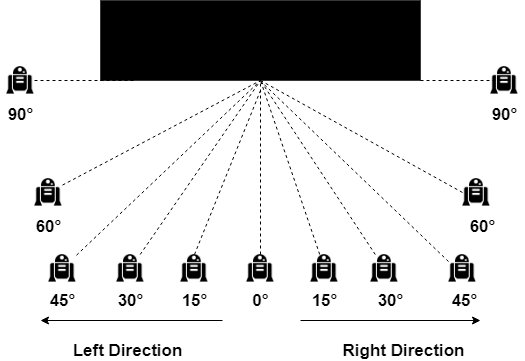
\includegraphics[width=12cm, height=7cm]{Degrees.png}
\textbf{Figure 1: Change of angle between the robot and the surface it is observing}
\end{center}
\end{enumerate}
\end{mdframed}
\vspace*{\baselineskip}

\subsection{Basic PID Controller}

The next step is to program the robot to position itself \emph{autonomously} at a set distance from
a vertical surface (such as a wall).  In order to do this you will need to implement a closed-loop
negative feedback system incorporating a PID controller.  The `reference input' $r$ corresponds to
the desired distance between the robot and the surface, the `feedback signal' $b$ corresponds to the
output of the ultrasonic distance sensor, and the `control signal' $u$ corresponds to the value that
is sent to the motors.  The PID controller should be of the form $u(t) = K_P e(t) + K_I \int e(t)dt
+ K_D \frac{de}{dt}(t)$ (as indicated earlier).

{\bfseries Note:}  \emph{You will have to measure $dt$ (the loop time) using the system clock.}

{\bfseries Note:}  \emph{Be aware that the \texttt{Lejos} EV3 library has separate commands to make
the motors go forwards or in reverse.  This means that you will have to convert $+ve$ and $-ve$
control signals into suitable motor commands.}

Once you have implemented the code, you should follow these steps:
\begin{enumerate}
	\item Set $r=50 cm$.
	\item Set $K_P=1$, $K_I=0$ and $K_D=0$.
	\item Place the robot 100 cm from a vertical surface with the ultrasonic sensor facing towards it.
	\item Run the code.
\end{enumerate}

If all is well, then your robot should move slowly towards the surface slowing down and eventually
stopping as it approaches the 50 cm point.

{\bfseries Note:}  \emph{If your robot appears to do the opposite of what you expect, try setting
$K_P=-1$.  If that solves the problem, then you have implemented a positive-feedback rather than a
negative-feedback loop.  This means that you need to swap the polarity of the signal being sent to
the motors (and reset $K_P=1$).}

Tick the following when your robot behaves correctly (by editing the \LaTeX\ source file, as
before):
\begin{todolist}
	\item[\done]  Robot behaves as expected
\end{todolist}

{\bfseries Question \myq:}  \emph{With the code still running, what happens if, after the robot has
arrived at the 50 cm point, you manually push it towards the surface?} (Worth up to 2 marks)\\
\begin{mdframed}
The robot will move backwards if it is manually pushed past the 50 cm point. The speed of the robot
moving backwards is directly proportional to the distance between the robot and the 50 cm point
after it has been pushed past the point, i.e. the robot will move backwards faster if it is closer
to the surface, and slower if it is far away from the surface and closer to the 50 cm point.
\end{mdframed}
\vspace*{\baselineskip}

Now implement an outer loop that swaps $r$ between 30 cm and 50 cm every 10 seconds.  As a result,
your robot should now change its position at regular intervals.  These step changes in $r$ will make
it easier to observe the robot's behaviour for different values of $K_P$, $K_I$ and $K_D$.

{\bfseries Question \myq:}  \emph{With $K_I=0$ and $K_D=0$, what happens when you experiment with
different values of $K_P$?  In particular, (i) what is a `good' value for $K_P$ (and why), (ii) what
value of $K_P$ causes the robot to start to oscillate continuously backwards and forwards around the
target $r$, and (iii) when it starts to oscillate continuously, what is the oscillation period?
Hint: start with $K_P =1$, then increase it gradually.} (Worth up to 5 marks)\\
\begin{mdframed}
\begin{enumerate}[label=(\roman*)]
  \item A `good' value of $K_P$ is the optimum value that allows the robot to arrive to the
    reference point quickly and accurately without overshooting and oscillating around the reference
    point. Any values lower than the `good' value will cause the robot to have higher stability,
    reaching the reference point more precisely at the cost of slower speed. Values larger than the
    `good' value will cause the robot to arrive quicker at the reference point, but the robot will
    have decreased stability where it will overshoot and have to correct it's position to arrive at
    the reference point. According to our experiment, $K_P = 75$ is a `good' value for our robot
    configuration. \par In the maze running competition, it might be better to use a slightly lower
    value of $K_P$ than the `good' value. This is because there is a slight delay in the WiFi
    connection between the robot and the computer. Hence, a slightly lower $K_P$ value will make the
    robot move slower and more stable as specified above. Also this can prevent the robot from
    running into the wall in the case of a short connection issue that is encountered throughout the
    run.
  \item We have experimented several values of `high' $K_P$ to find out the `ultimate gain'.
\begin{itemize}
\item When $K_P = 103$, the robot started to oscillate slowly around the reference point, but it
eventually converged and stopped.
\item When $K_P = 125$, the robot oscillated consistently around the reference point.
\item When $K_P = 155$, the robot oscillated heavily around the reference point, the oscillation
distance became larger and larger overtime.
\end{itemize}
  Hence, our `ultimate gain' $K_U = 125$.
\item When $K_P = 125$, the robot oscillated 7 times in 10 seconds. Therefore, the oscillation
period $T_U$ is \( \frac{10}{7} \) = 1.4286 secs.
\end{enumerate}
\end{mdframed}
\vspace*{\baselineskip}

The value of $K_P$ that causes the robot to oscillate backwards and forwards continuously is known
as the `ultimate gain' $K_U$, and the oscillation period is designated as $T_U$.

{\bfseries Note:}  \emph{Be aware that $T_U$ is a measure of time, not frequency.  I.e.\ if the
robot oscillates backwards and forwards at a rate of five times a second, then $T_U=1/5=0.2$ secs.}

{\bfseries Question \myq:}  \emph{What is the relationship between the `good' value of $K_P$ that
you discovered by experimentation and the value of $K_U$ that you measured?} (Worth up to 5 marks)\\
\begin{mdframed}
The value of $K_U$ is much higher than the `good' $K_P$ value. This is because the value of $K_P$ is
inversely proportional to the stability of the robot. Assuming $K_I$ and $K_D$ are zero, when the
value of $K_P$ would be very small, the robot would move very slowly towards the reference point and
stop exactly when it reaches the reference point. The `good' value of $K_P$ that we discovered is a
compromise between speed and accuracy so that the robot reaches the set reference point quickly
enough stopping on the reference point accurately without oscillating. Our $K_U$ shows the point
where the compromise mentioned previously is more inclined towards the speed of the robot, so the
robot reaches the reference point very fast but will not be able to precisely stop at the required
distance so it will start to oscillate back and fourth around it.
\end{mdframed}
 \vspace*{\baselineskip}


\subsection {PID Tuning}

There are several methods available for tuning the parameters of a PID controller.  The
\emph{manual} method involves setting $K_P=0.5K_U$, $K_I=0$ and $K_D=0$.  Next, $K_I$ is gradually
increased to improve the convergence.  Then $K_D$ is gradually increased to improve the
responsiveness.

A more formal tuning approach is known as the \emph{Ziegler-Nichols} method.  Once $K_U$ and $T_U$
have been determined, the PID gains may be set according to the following heuristic:
\begin{center}
	\begin{tabular}{ | c | c | c | c | } \hline
		 & \bf{$K_P$} & \bf{$K_I$} & \bf{$K_D$} \\ \hline
		\bf{P} & $0.5K_U$ &  &  \\ \hline
		\bf{PI} & $0.45K_U$ & $0.54K_U/T_U$ &  \\ \hline
		\bf{PID} & $0.6K_U$ & $1.2K_U/T_U$ & $3K_UT_U/40$ \\ \hline
	\end{tabular}
\end{center}
\vspace*{\baselineskip}

{\bfseries Question \myq:}  \emph{What values of $K_P$, $K_I$ and $K_D$ are given by the
Ziegler-Nichols method for a P, PI and PID controller (based on the values of $K_U$ and $T_U$ you
measured previously)?} (Worth up to 5 marks)\\
\begin{mdframed}
When $K_U = 125$ and $T_U = 1.4286$,
\begin{center}
	\begin{tabular}{ | c | c | c | c | } \hline
		 & \bf{$K_P$} & \bf{$K_I$} & \bf{$K_D$} \\ \hline
		\bf{P} & 62.5 &  &  \\ \hline
		\bf{PI} & 56.25 & 47.2491 &  \\ \hline
		\bf{PID} & 75 & 104.9979 & 13.3931 \\ \hline
	\end{tabular}
\end{center}
\vspace{3mm}
\begin{center}
\textbf{Table 4. Values of $K_P$, $K_I$ and $K_D$ for a P, PI and PID controller using Ziegler-Nichols method}
\end{center}

The values of $K_P$, $K_I$ and $K_D$ given by the Ziegler-Nichols method do not give perfect results
on our robot. We were required to perform a manual tuning process on $K_P$, $K_I$ and $K_D$ by
trial-and-error. According to our experimentation, the values of $K_P$ and $K_I$ given by
Ziegler-Nichols method were too high. Using the values of $K_P$, $K_I$ and $K_D$ in \textbf{Table 4}
caused the robot to  speed up and stop suddenly at certain point. Although the robot moved quickly
to the target, its movement was too unpredictable that it would be risky to use these values in the
maze competition.

\par We managed to get the optimal values of $K_P$, $K_I$ and $K_D$ for our robot by lowering $K_P$
and $K_I$ drastically, and changing the formula we used to set the speed of the motors. Since we
converted the distance returned by the sensors to centimetres, we are required to apply a multiplier
to one of the motors in order to make the robot turn effectively. The final values are $K_P = 40$.
$K_I = 10$ and $K_D = 13$.
\end{mdframed}
\vspace*{\baselineskip}

Confirm the effectiveness of the Ziegler-Nichols method by setting the values for $K_P$, $K_I$ and
$K_D$ in your controller, and tick the following:
\begin{todolist}
	\item[\done] The robot moves quickly to the target and stops with minimal overshoot
 \end{todolist}

{\bfseries Question \myq:}  \emph{Using the values for $K_P$, $K_I$ and $K_D$ given by the
Ziegler-Nichols method, what happens when you decrease the sampling rate (e.g.\ by introducing a
`wait' function in the loop)?  What is the significance of your observations?} (Worth up to 5
marks)\\
\begin{mdframed}
Using the values for $K_P$, $K_I$ and $K_D$ given by the Ziegler-Nichols method above, \textbf{Table
5} below shows the experimented wait periods and their result.
\begin{center}
\begin{tabular}{|P{3cm}|P{9cm}|}\hline
Wait period (second) & Result                                                                                                                                                                                                                                                                                 \\ \hline
0.1                  & The robot was still able to function accurately. It might slightly overshoot the reference point, depending on the initial distance between the robot and the reference point, but the difference between a continuous sampling rate is hardly noticeable.                                \\ \hline
0.2                  & The overshoot was more obvious, but the robot reached the reference point slightly quicker due to the delay in the speed change. The robot started to oscillate slowly around the reference point after it reached it, and eventually converged. It is still considered as functioning. \\ \hline
0.3                  & The robot reached the reference point quicker than the previous setting, but the overshoot became worse. The oscillation becomes larger and inconsistent. The control quality of the robot starts to degrade.                                                                           \\ \hline
0.4                  & The robot maintained its initial speed until it was very close to the reference point, and the sudden change of the speed is obvious. The overshoot and oscillation was more inconsistent than the previous setting.                                                                    \\ \hline
0.5                  & The robot will always overshoot the reference point. The distance between the robot and the reference point was always different when the wait period was over.                                                                                                                         \\ \hline
\end{tabular}
\end{center}
\vspace{3mm}
\begin{center}
\textbf{Table 5: Experimentations of different wait periods and their results}
\end{center}

Introducing a `wait' function in the loop had a negative effect on the performance of our robot and
degraded the control quality. This is due to the fact that we have decreased the sampling rate and
the robot had less values to work with. During the `wait' periods,   the robot is not receiving the
feedback from the sensors, hence, its state (moving or stationary) would not be changed because no
control signal is produced during the `wait' periods. Therefore, it would be unaware of its position
for a longer period of time, making it more likely to overshoot the set reference point and
oscillate around it. In order to increase the control quality of our PID controller we have to
adjust the $K_P$ value so that the decrease in sampling rate will be accounted for.

According to our experimentations for a 0.1 seconds wait period, the `ultimate gain' $K_U$ is now
120. The robot oscillated 13 times in 20 seconds, so the oscillation period $T_U$ is \(
\frac{20}{13} \) = 1.5385 secs. Hence, the values for $K_P$, $K_I$ and $K_D$ with a 0.1 seconds wait
period are
\begin{center}
	\begin{tabular}{ | c | c | c | c | } \hline
		 & \bf{$K_P$} & \bf{$K_I$} & \bf{$K_D$} \\ \hline
		\bf{P} & 60 &  &  \\ \hline
		\bf{PI} & 54 & 42.12 &  \\ \hline
		\bf{PID} & 72 & 93.6 & 13.8462 \\ \hline
	\end{tabular}
\end{center}
\vspace{3mm}
\begin{center}
\textbf{Table 6: Values of $K_P$, $K_I$ and $K_D$ for a P, PI and PID controller using
Ziegler-Nichols method when the wait period is 0.1 seconds}
\end{center}

According to the table above, it can be stated that the values of $K_P$, $K_I$ decreases and $K_D$
increases as the wait period increases.

\par In the maze running competition, it is best to use the highest sampling rate available. This is
because the surroundings of the robot change too frequently. The robot needs to maintain the
distance between itself and two walls, and also needs to turn accordingly when there is a curve in
the maze.
\end{mdframed}
\vspace*{\baselineskip}


\subsection{PID-based Steering}

Finally (for Part I), reposition your ultrasonic sensor so that it faces sideways from the robot.

Now re-program your robot with a PID controller that maintains a fixed distance from a wall as the
robot travels along parallel to it.  This will require the speed to be set at some fixed value, and
the PID-based control loop will handle the steering.  Use the Ziegler-Nichols method to determine
appropriate values for $K_P$, $K_I$ and $K_D$ (this can be done while the robot is stationary and
changing the target distance a few centimetres once every 10 seconds, as before).

{\bfseries Note:}  \emph{It is particularly important that the sensor is mounted well forward of the
driving wheels, otherwise it will not be sensitive to changes in direction when the robot is
stationary.}

{\bfseries Question \myq:}  \emph{What values for $K_U$ and $T_U$ did you measure, and what are the
resulting values for $K_P$, $K_I$ and $K_D$  given by the Ziegler-Nichols method?} (Worth up to 5
marks)\\
\begin{mdframed}
We have set the base speed of the robot as 200 and positioned the ultrasonic sensor at the left side
of the robot. We measured the value of $K_P$ using this setting.

The `good' value of $K_P$ measured was 83, and the `ultimate gain' $K_U$ measured was 140. The robot
oscillated 8 times in 5 seconds, hence the oscillation period $T_U$ is \( \frac{5}{4} \) = 1.25
secs.

When $K_U = 140$ and $T_U = 1.25$,
\begin{center}
	\begin{tabular}{ | c | c | c | c | } \hline
		 & \bf{$K_P$} & \bf{$K_I$} & \bf{$K_D$} \\ \hline
		\bf{P} & 70 &  &  \\ \hline
		\bf{PI} & 63 & 60.48 &  \\ \hline
		\bf{PID} & 84 & 134.4 & 13.125 \\ \hline
	\end{tabular}
\end{center}
\vspace{3mm}
\begin{center}
\textbf{Table 7: Values of $K_P$, $K_I$ and $K_D$ for a P, PI and PID controller using Ziegler-Nichols method for left wall steering}
\end{center}

Similar to \textbf{Question 10}, these $K_P$, $K_I$ and $K_D$ values given by Zielger-Nichols method
did not produce satisfying result. The robot turned too quickly to right when it passed the
reference value, and turned too quickly back to left again, causing the robot to move in a
snake-like movement.
\end{mdframed}
\vspace*{\baselineskip}

Confirm the effectiveness of these values for $K_P$, $K_I$ and $K_D$, and tick the following:
\begin{todolist}
	\item[\done] The robot travels along a wall maintaining a constant distance from it
\end{todolist}


\subsection{Summary}

You have successfully completed Part I of the assignment, and you should now have all of the skills
necessary to move on to Part II.


\newpage
\section{Part II: Maze-Running Competition}

\subsection{Objective}

The aim of Part II of the assignment is to combine the theoretical knowledge you have obtained in
the lectures with the practical experience you have acquired in Part I to design and implement a
robot that is capable of competing in a simple maze-running competition.

The challenge is to navigate a corridor (that will be set up in the robot arena) in the fastest time
possible and without touching the walls.  The precise layout will not be revealed until the final
lab session.  However, you will be able to practice in the arena beforehand.  The two walls of the
corridor are painted different colours so that, if necessary, your robot can determine if it is
going in the correct direction.

You need to decide which control principle(s) to use and how to set up your robot's sensors and
actuators.  Also, since it's a competition, you will need to to think about how your robot manages
`risk', i.e.\ is it better to be slow-and-careful or reckless-but-fast?  You will probably need to
experiment with various alternatives before deciding on a final approach.

{\bfseries Note:}  \emph{You will need to adopt good working practices for (i) organising your team
and (ii) software version control.  The latter is important as robots are notorious for failing
after a so-called `improvement', so being able to revert easily to an earlier version will save a
lot of pain and grief.}

{\bfseries Note:}  \emph{Each Lego kit contains two ultrasonic sensors.}

{\bfseries Note:}  \emph{The maze will be a simple winding corridor.  There will be no dead-ends, no
loops and no junctions.  However, there may be chicanes and small breaks in the wall.}


\subsection{The Competition}

In order to give every team an equal chance, the competition will be organised into a number of
leagues, each consisting of several teams (and their robots).  Marks will be awarded based on each
robot's performance \textbf{within its league}.  This will mean that each team will be competing
against teams that have had an equal amount of time devoted to the development of their respective
robots.  The competition will take place during the final lab session.

{\bfseries Note:}  \emph{If there is time at the end of the league battles, the winning robot in
each league will compete again to find the overall champion.  This `championship' contest will not
count towards the marks for the assignment, but a (small) prize may be awarded.}

As you can imagine, running such an event with a large number of teams/robots requires very precise
time management, so we will be issuing a strict timetable for the final lab session.  This should
appear on MOLE the week before.  It is essential that you prepare carefully for your designated time
slot (otherwise you may lose marks - see below).

The rules for the competition are as follows:
\begin{enumerate}
	\item Any number of practice runs may be made (subject to the availability of the arena).
	\item Each team must register their arrival at the arena (with their robot) 10 mins prior to their
	league's designated time slot, after which no further technical development will be permitted.
	\item Each team will be called forward in turn to place their robot on the starting line.
	\item An `official' run for each team's robot will be timed by the lab demonstrators.
	\item If a robot fails to complete a run within a \textbf{3 minute time limit}, the demonstrators
	will record the furthest position it reached.
	\item It is permitted for a designated team member to rescue their robot and place it back on the
	course at the place where things went wrong \textbf{twice} per run without penalty, but the clock
	will keep running.  A third rescue is not permitted, instead the run will be terminated and the
	position reached will be recorded.
	\item Failure to arrive at the arena at the designated time will earn a penalty (see below) and
	may mean that you do not get a run.
\end{enumerate}

Marks will be awarded as follows:
\begin{itemize}
	\item 5 marks will be awarded for a run completed within the 3 minute time limit.
	\item 5 marks will be awarded for a `clean' run. (i.e.\ no walls touched and no rescues).
	\item 10 marks will be awarded to the team with the best run within their league, 9 marks to the
	second best team, and so on.  A team who fails to arrive at the arena at their designated time
	will be ranked last in their league.
\end{itemize}

{\bfseries Question \myq:}  \emph{What was the result of your official attempt?} (Worth up to 20
marks)\\
\begin{mdframed}
\begin{center}
	\begin{tabular}{ |c|c|c|c|c|c|c| } \hline
		 \bf{Completed} & \bf{Wall Touches} & \bf{Rescues} & \bf{Time} & \bf{Distance} & \bf{Rank} \\
		 \hline
		Y & 1 & 1 & 00:01:02 & 10.5 metres & 2nd \\ \hline
	\end{tabular}
\end{center}
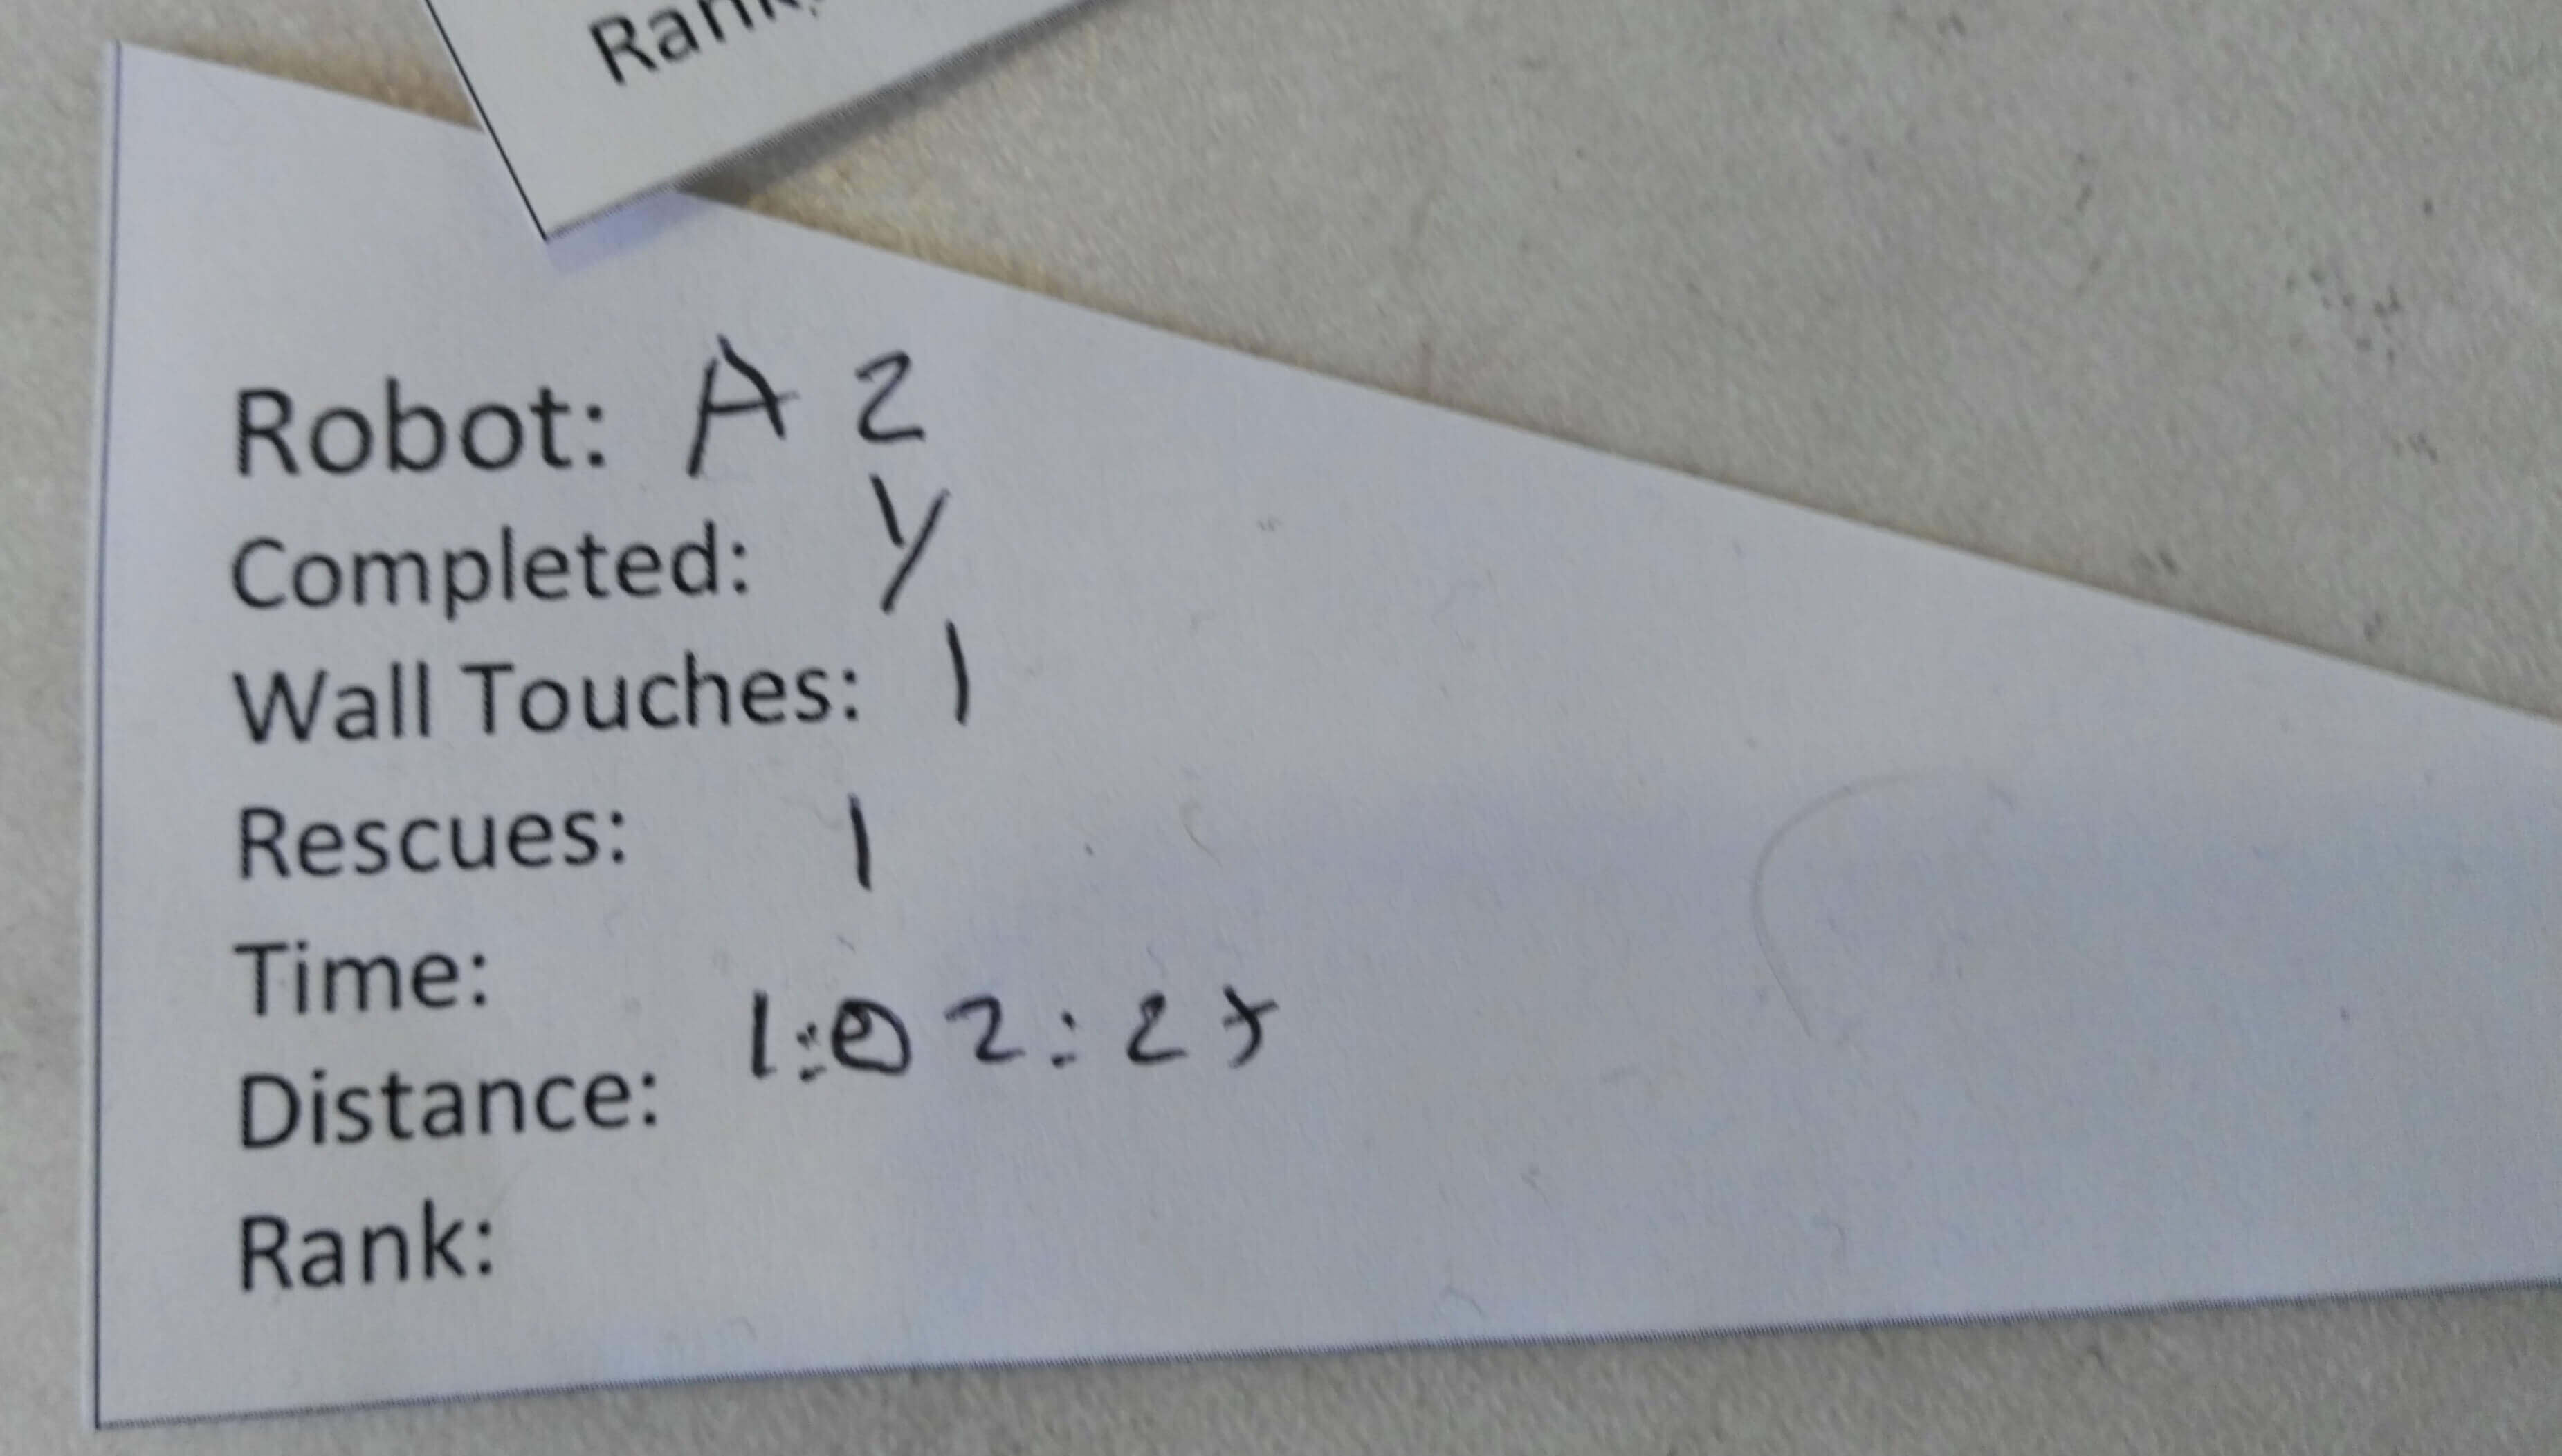
\includegraphics[width=\textwidth]{result.jpg}

Our actual score is 00:01:17 with the time penalty added due to rescue and wall touch.
\end{mdframed}
\vspace*{\baselineskip}


\subsection{Your Team's Solution}

{\bfseries Question \myq:}  \emph{In terms of your robot's software architecture, what principles
did you explore, and what was the final approach taken (include a system diagram)?} (Worth up to 15
marks)\\
\begin{mdframed}
\begin{center}
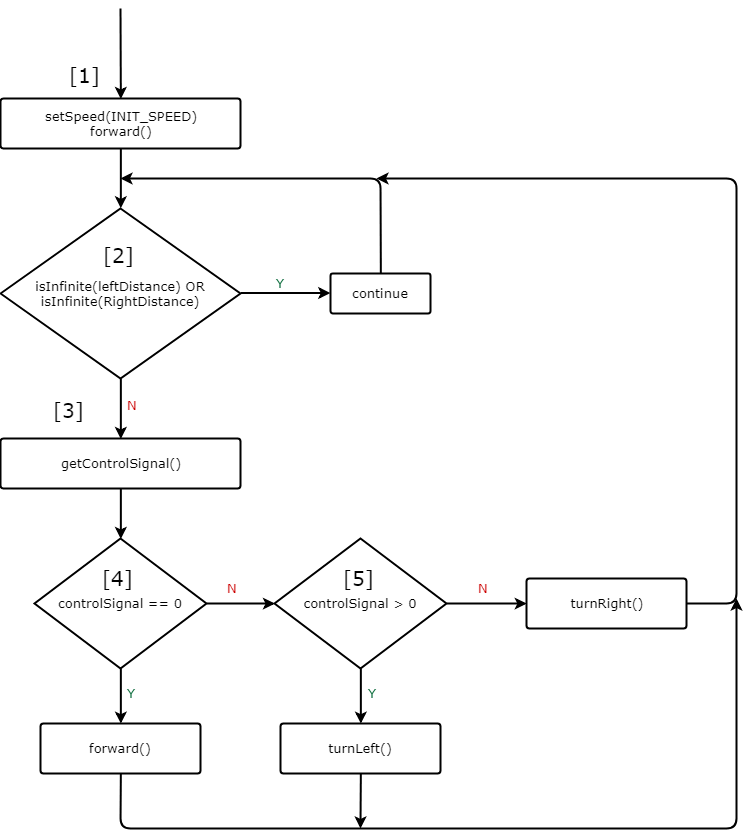
\includegraphics[width=14cm]{flowchart.png}
\textbf{Figure 2. Flowchart of our robot control loop}
\end{center}

\begin{enumerate}
\item Step [1]: Before entering the loop, the initial speed of the robot is set at a fixed value and
it is set to move forward.
\item Step [2]: If the left sensor or the right sensor detects an \emph{Infinity} distance, the
control loop is skipped and the robot will continue its last action (forward, turn left, or turn
right)
\item Step [3]: Our `error signal' $e$ is defined as \emph{leftDistance - rightDistance}, where
\emph{leftDistance} is the distance returned by the left sensor and vice versa. The formula for
calculating the `control signal' $u$ is:
\begin{center}
($K_P$ $\times$ error) + ($K_I$ $\times$ integral) + ($K_D$ $\times$ derivative)
\end{center}
where integral = $\frac{2}{3} \times $(integral + error), derivative = error - lastError
\item Step [4]: If the control signal $u = 0$, then the robot should move forward.
\item Step [5]: If the control signal $u > 0$, which means \emph{leftDistance $>$ rightDistance},
then the robot should turn left. Else the robot should turn right because \emph{leftDistance $<$
rightDistance}.
\end{enumerate}

Our final system design is shown in \textbf{Figure 2}, showing the decisions robot continuously
loops through. It sees which direction it needs to turn by comparing the \emph{leftDistance} and
\emph{rightDistance} in order to find an equilibrium between the two walls, adjusts its course to do
so, then loops again to smoothly make its way through the course. In the case of detecting an
\emph{Infinity} value, the robot will continue its last action as it is unable to determine whether
that is just a disturbance or a sharp turn. Overall, this final approach is more stable and
practical than having multiple \emph{if else} statements in the code to control the robot actions.

\begin{center}
  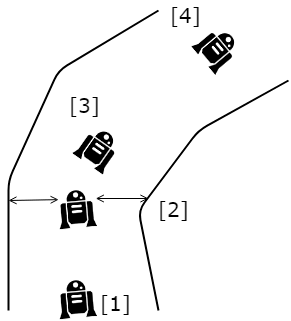
\includegraphics[width=5cm]{final_illustration.png}\\
  \textbf{Figure 3: Robot movement for a turn in final our implementation}
\end{center}

As shown in \textbf{Figure 3}, our final implementation will allow the robot to maintain an equal
distance between the left and right wall. At \textbf{[1]}, the robot will be moving forward since
the left and right sensor detected the same distance. At \textbf{[2]}, the \emph{rightDistance} is
now larger than the \emph{leftDistance}. According to the control loop, the control signal $u$ is
now less than 0, so the robot should be turning right. At \textbf{[3]}, after the robot has turned
right, it will try to maintain an equal distance between the left and right wall again. At
\textbf{[4]}, the robot has completed the turn, everything is back to the same state as \textbf{[1]}
again.

At first, we investigated a variety of PID controller implementations in order to gather a better
insight as to what would be the best approach for our specific scenario. From our research we
established that our implementation would consist of trying to maintain an equilibrium between a set
reference point and the wall. By doing this we would attempt to follow one of the walls the whole
way round the maze to get to the end. After experimenting with a few difference distances from the
wall it was found that sometimes this approach did not work correctly. When following a wall, the
robot would get stuck when the angle was less than \ang{90} or there was a very sharp turn. This was
due to the fact that the robot was not able to predict the turn because of the software
implementation and because it uses an input only to sense the distance to the side wall and and has
no real knowledge of anything ahead. Using \textbf{Figure 4} we can envisage the scenario better and
show that when the angle of the turn is less than \ang{90}, the robot will be unable to take the
turn using this method.
\vspace*{\baselineskip}
\begin{center}
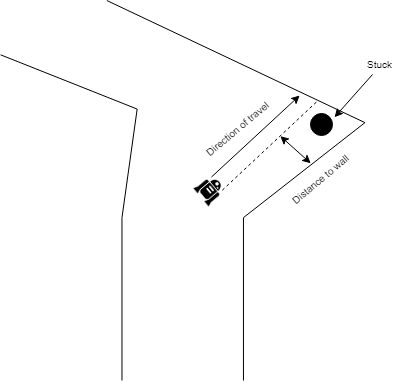
\includegraphics[width=13cm, height=10cm]{OneWall.png}
\textbf{Figure 4: First implementation attempt}
\end{center}
Originally in \textbf{Step[5]} of \textbf{Figure 2}, we implemented a function that compared the
last distances returned and the current distance returned by  the sensors. For example, if the
difference between the \emph{lastDistance} and \emph{currentDistance} returned by the left sensor
exceeds a certain threshold, then the robot knows that it has reached a sharp turn, and it should
keep turning left until the control signal becomes 0. Theoretically, this approach should prevent
the case where the robot does not turn enough in a sharp turn. However, due to the delay in the WiFi
connection, the lag in readings received caused the robot to continue turning for too long, hitting
the wall.

Our second approach was to change our implementation slightly and attempt to monitor the
distance between the left and the right walls simultaneously. Using this method, displayed in
\textbf{Figure 5}, we tried to keep the robot in between the two walls by keeping the difference
between the distances of the robot and each of the two walls at 0 throughout the run in the maze.
This approach turned out to solve the problem that we encountered previously, therefore now even if
our robot encounters a very sharp turn it will be able to cope with it. This is because the robot
will never be too close to the wall at any point which will allow plenty of time and distance to
complete the turn for any sharp corners encountered. The only slight problem with this approach was
that using the previous values for the configuration of the PID Controller would not work anymore.
Therefore in order to solve this we had to experiment further so that we can find the correct PID
configuration variables.
\vspace*{\baselineskip}
\begin{center}
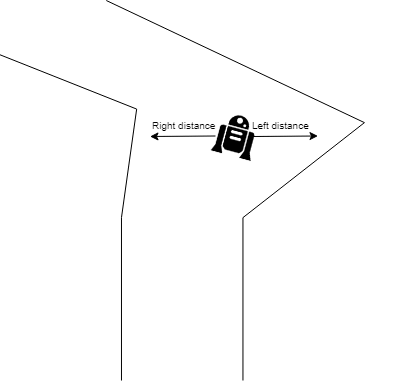
\includegraphics[width=13cm, height=10cm]{TwoWall.png}
\textbf{Figure 5: Second implementation attempt}
\end{center}

\begin{center}
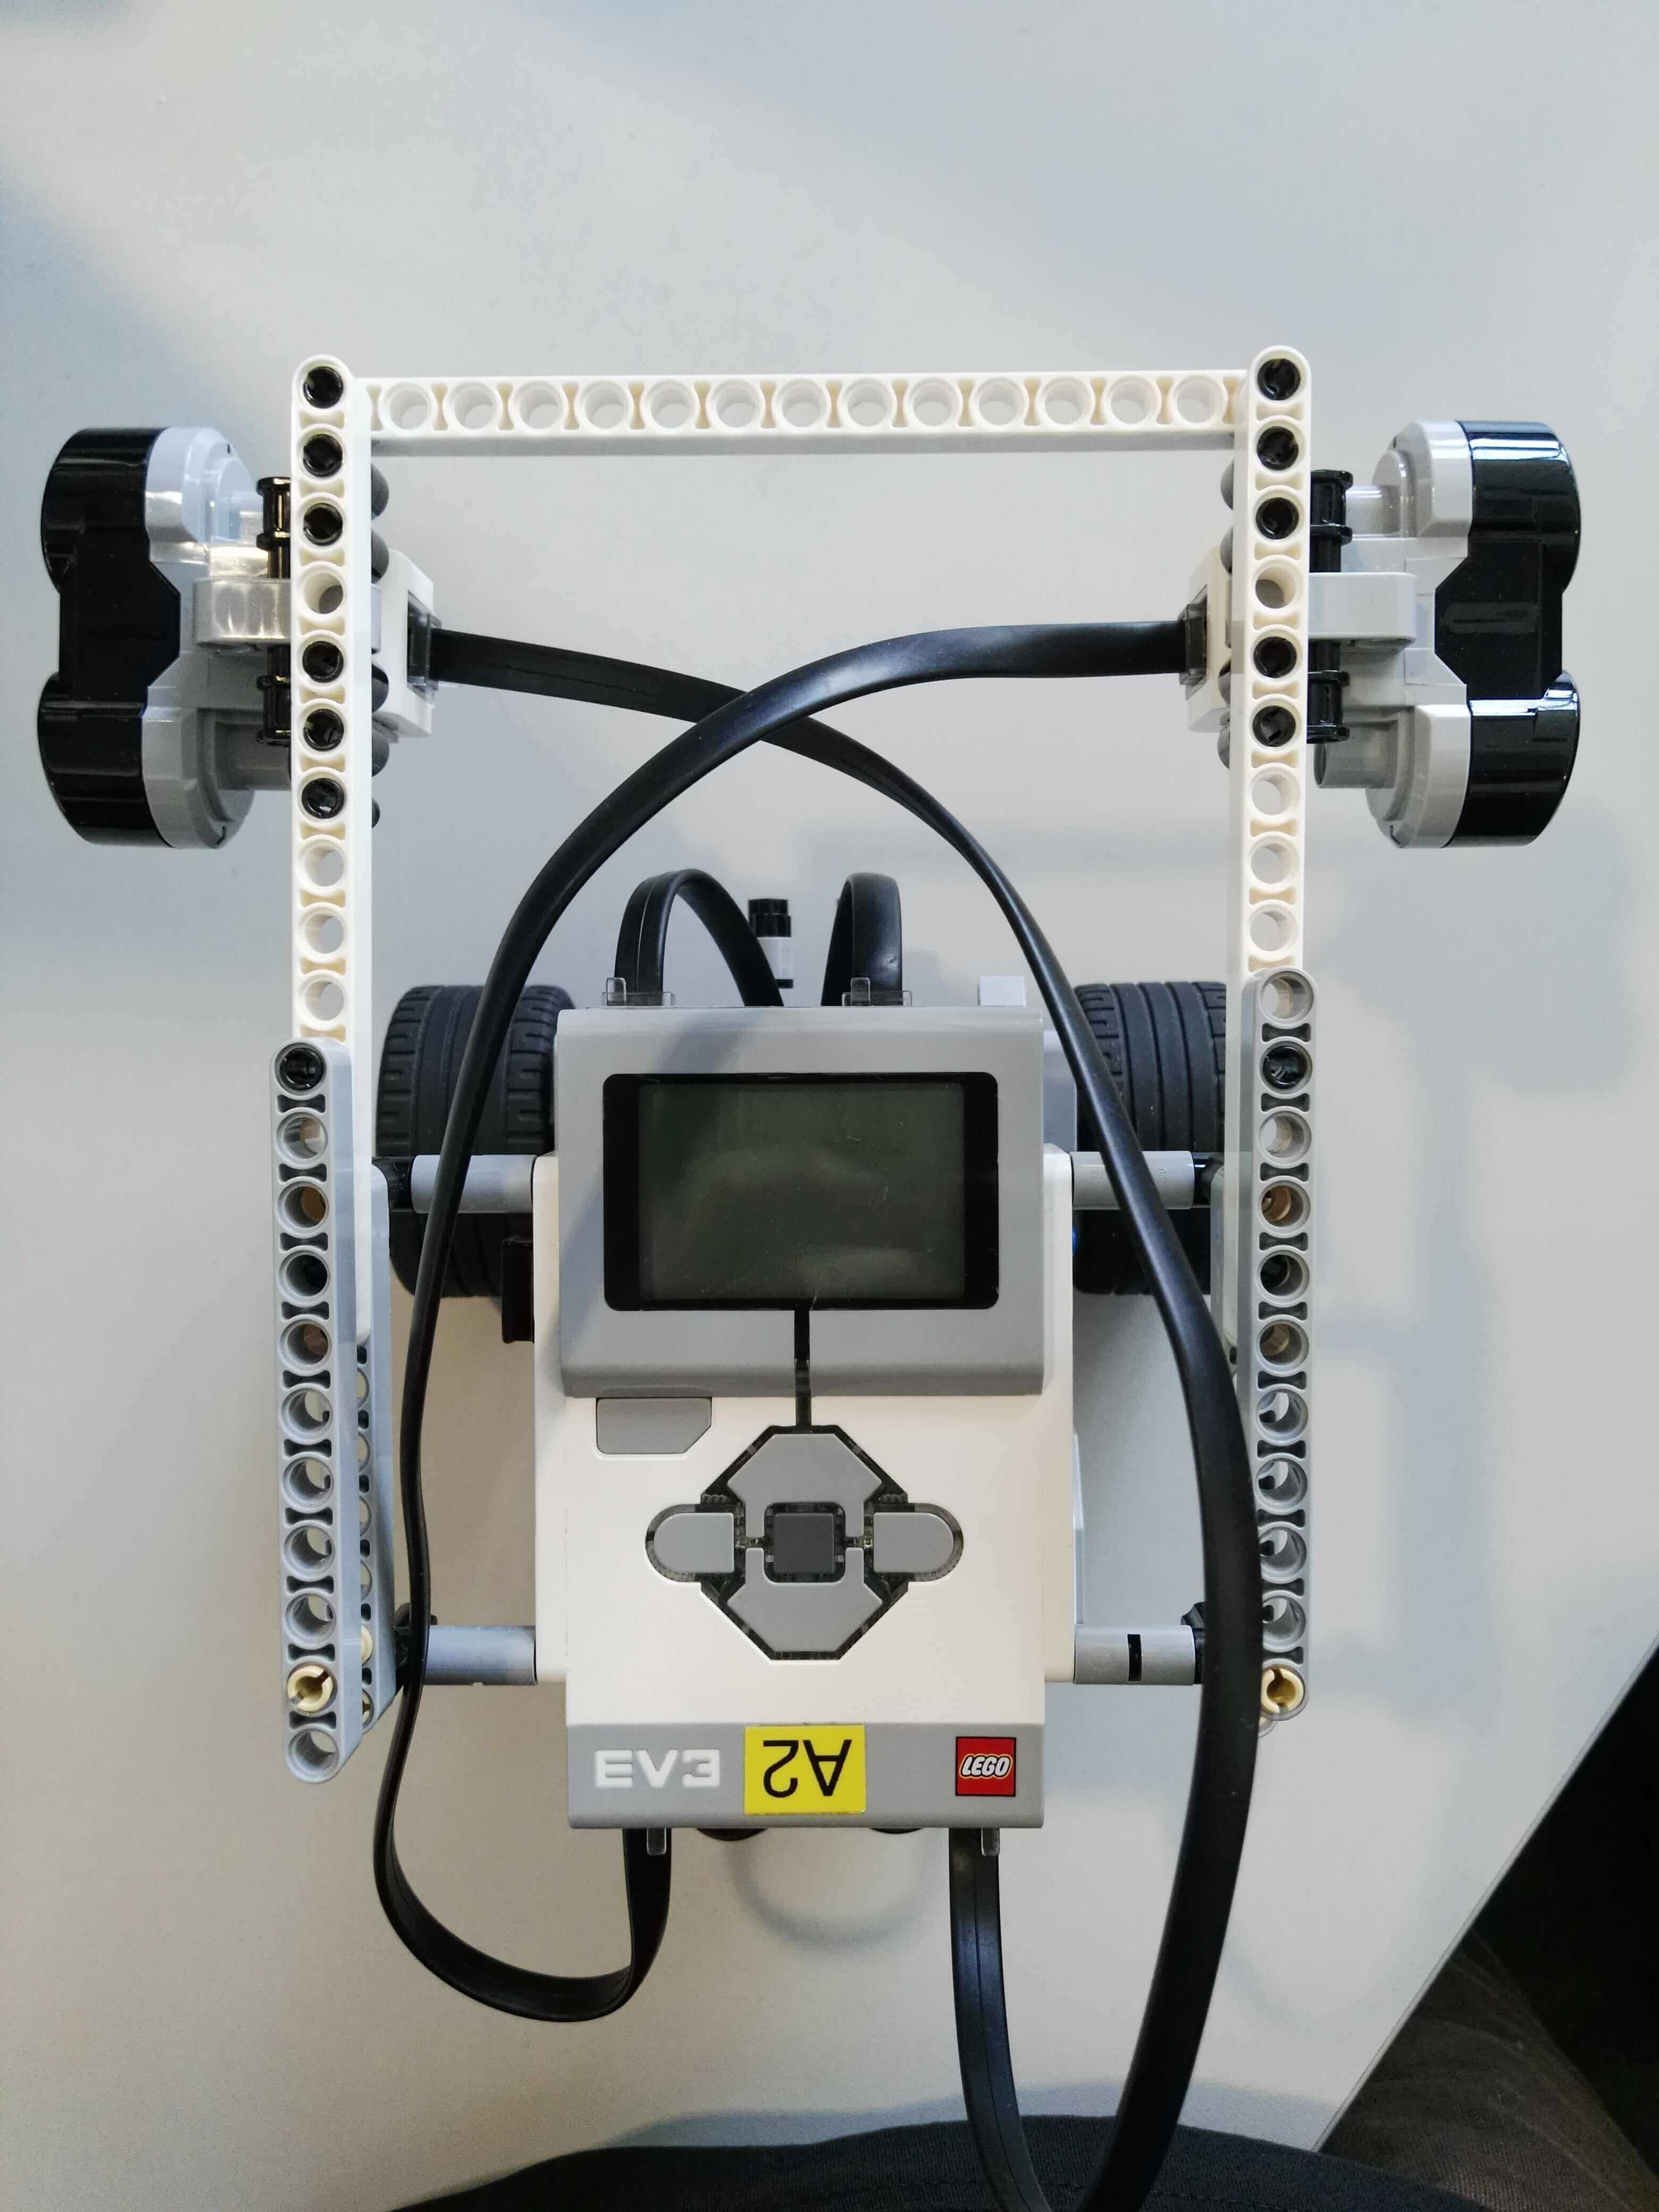
\includegraphics[width=4.5cm]{horizontal1.jpg}
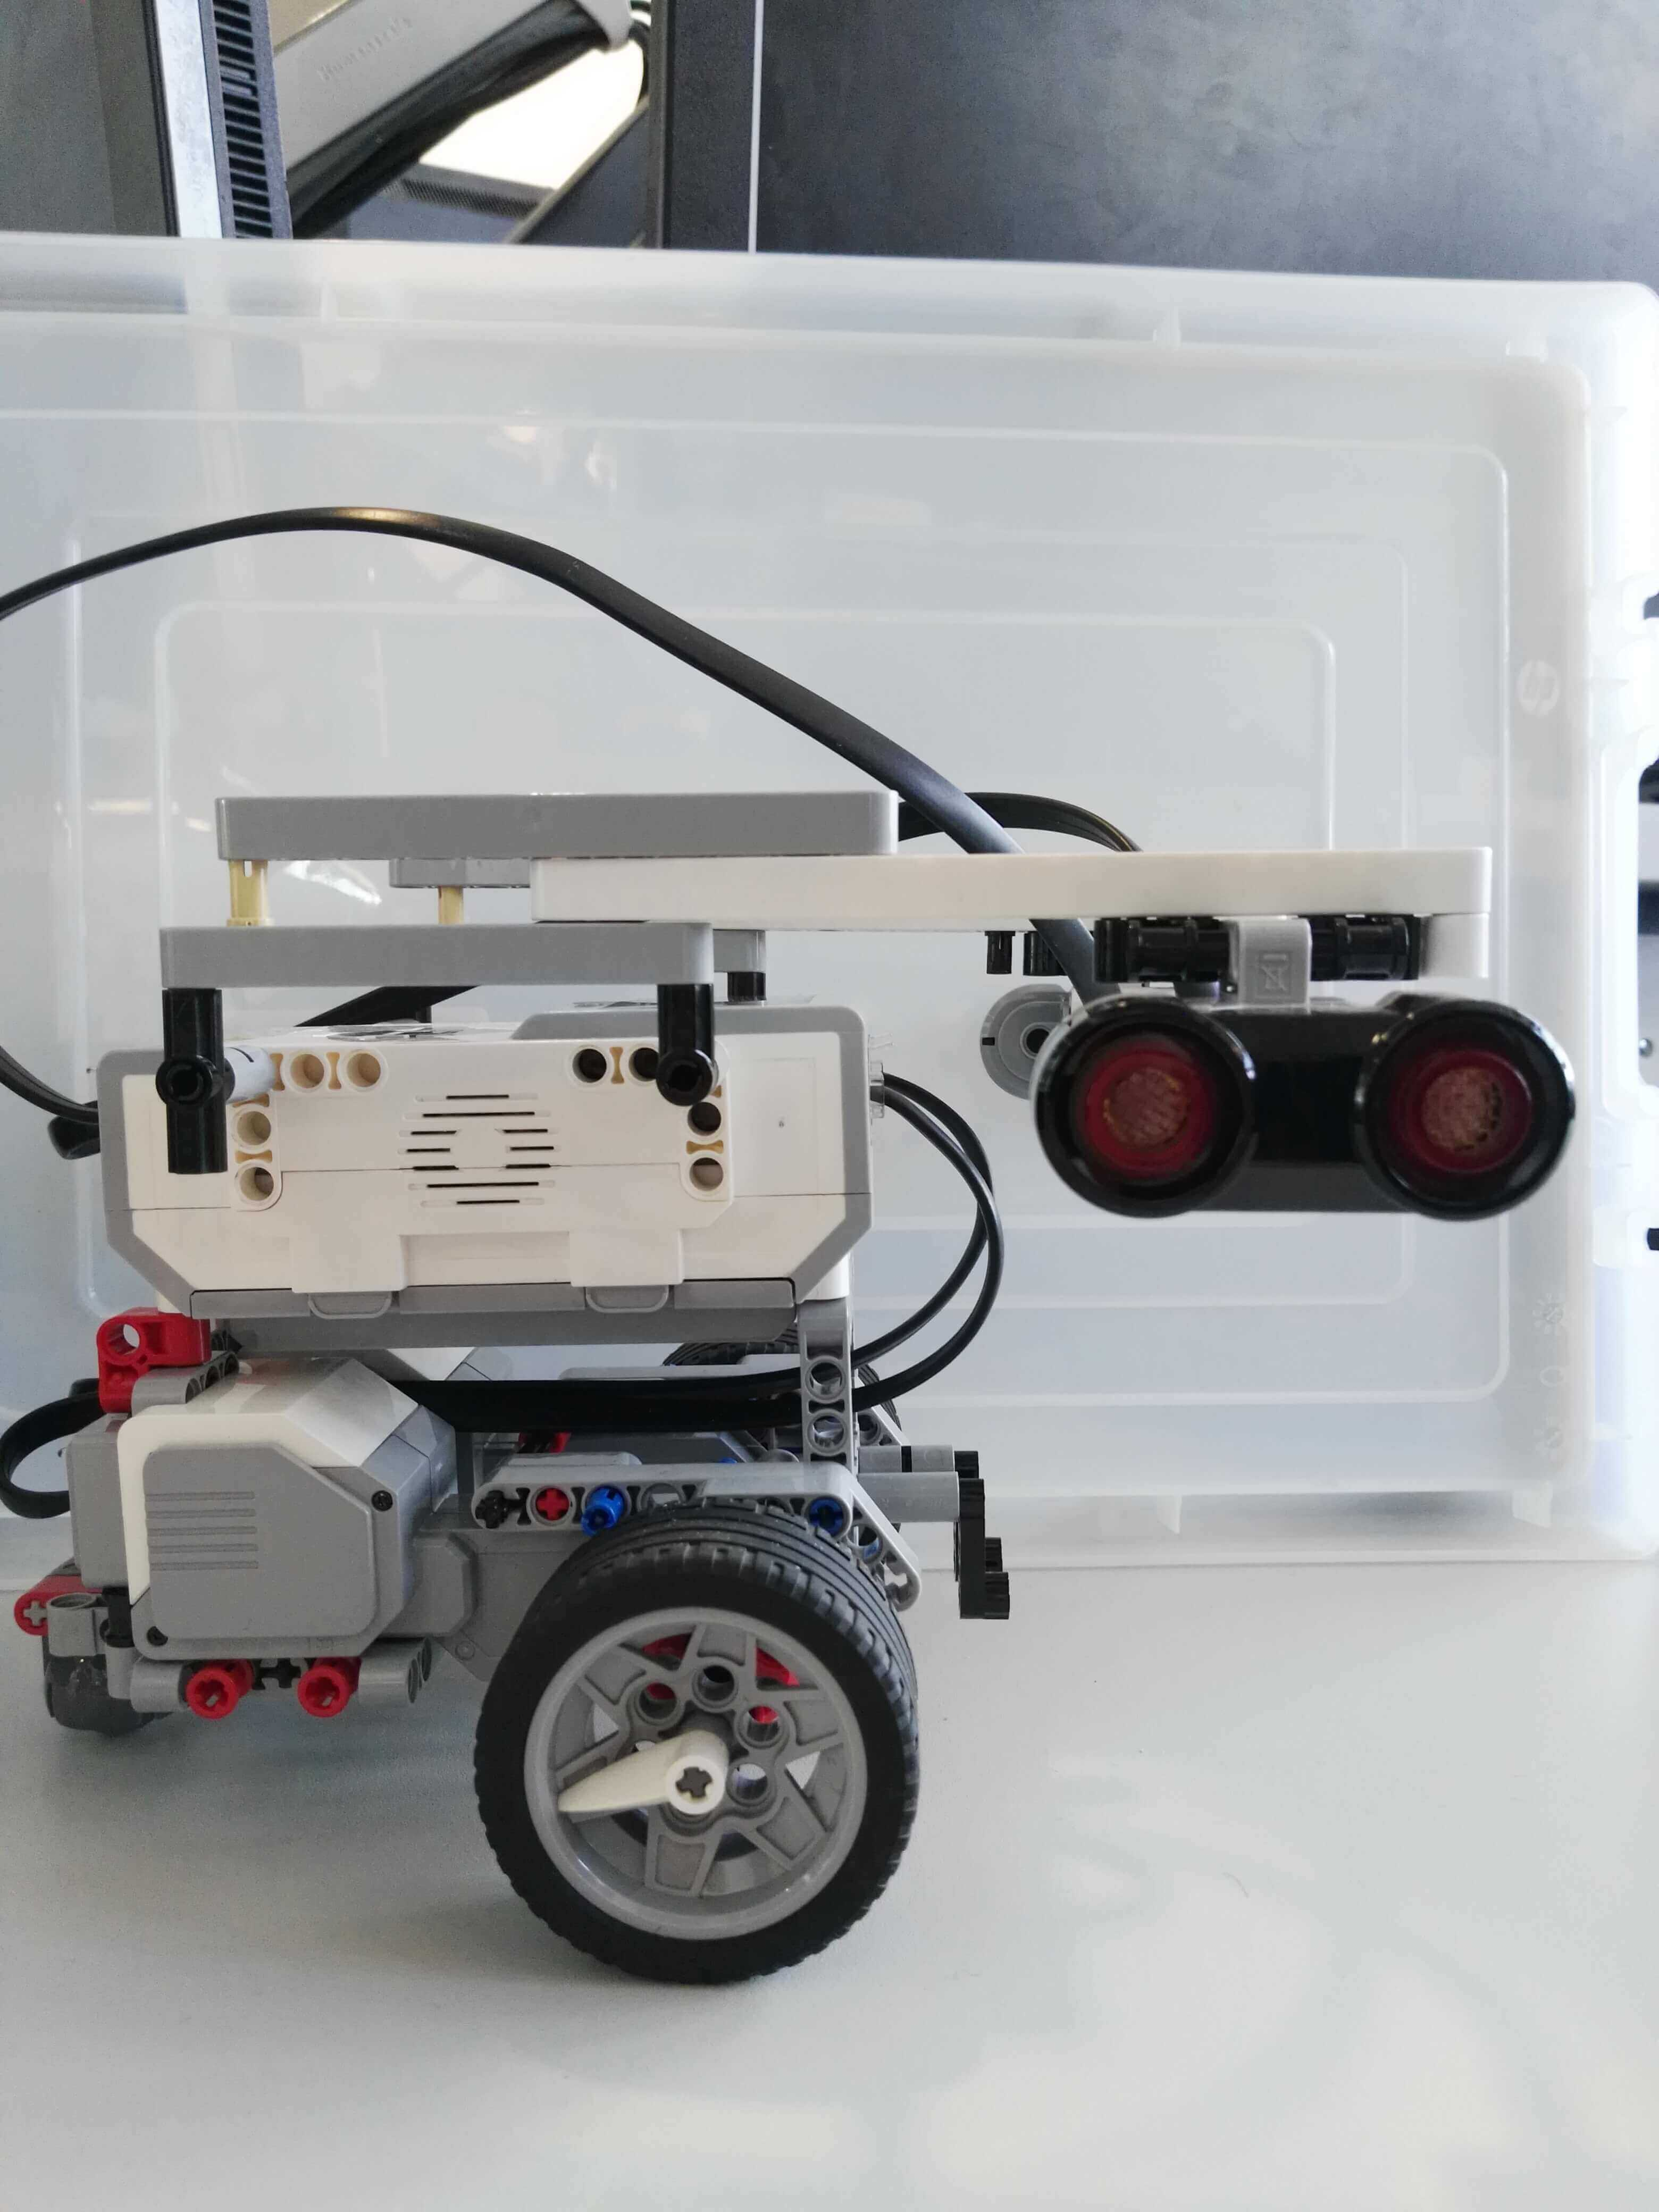
\includegraphics[width=4.5cm]{horizontal2.jpg}
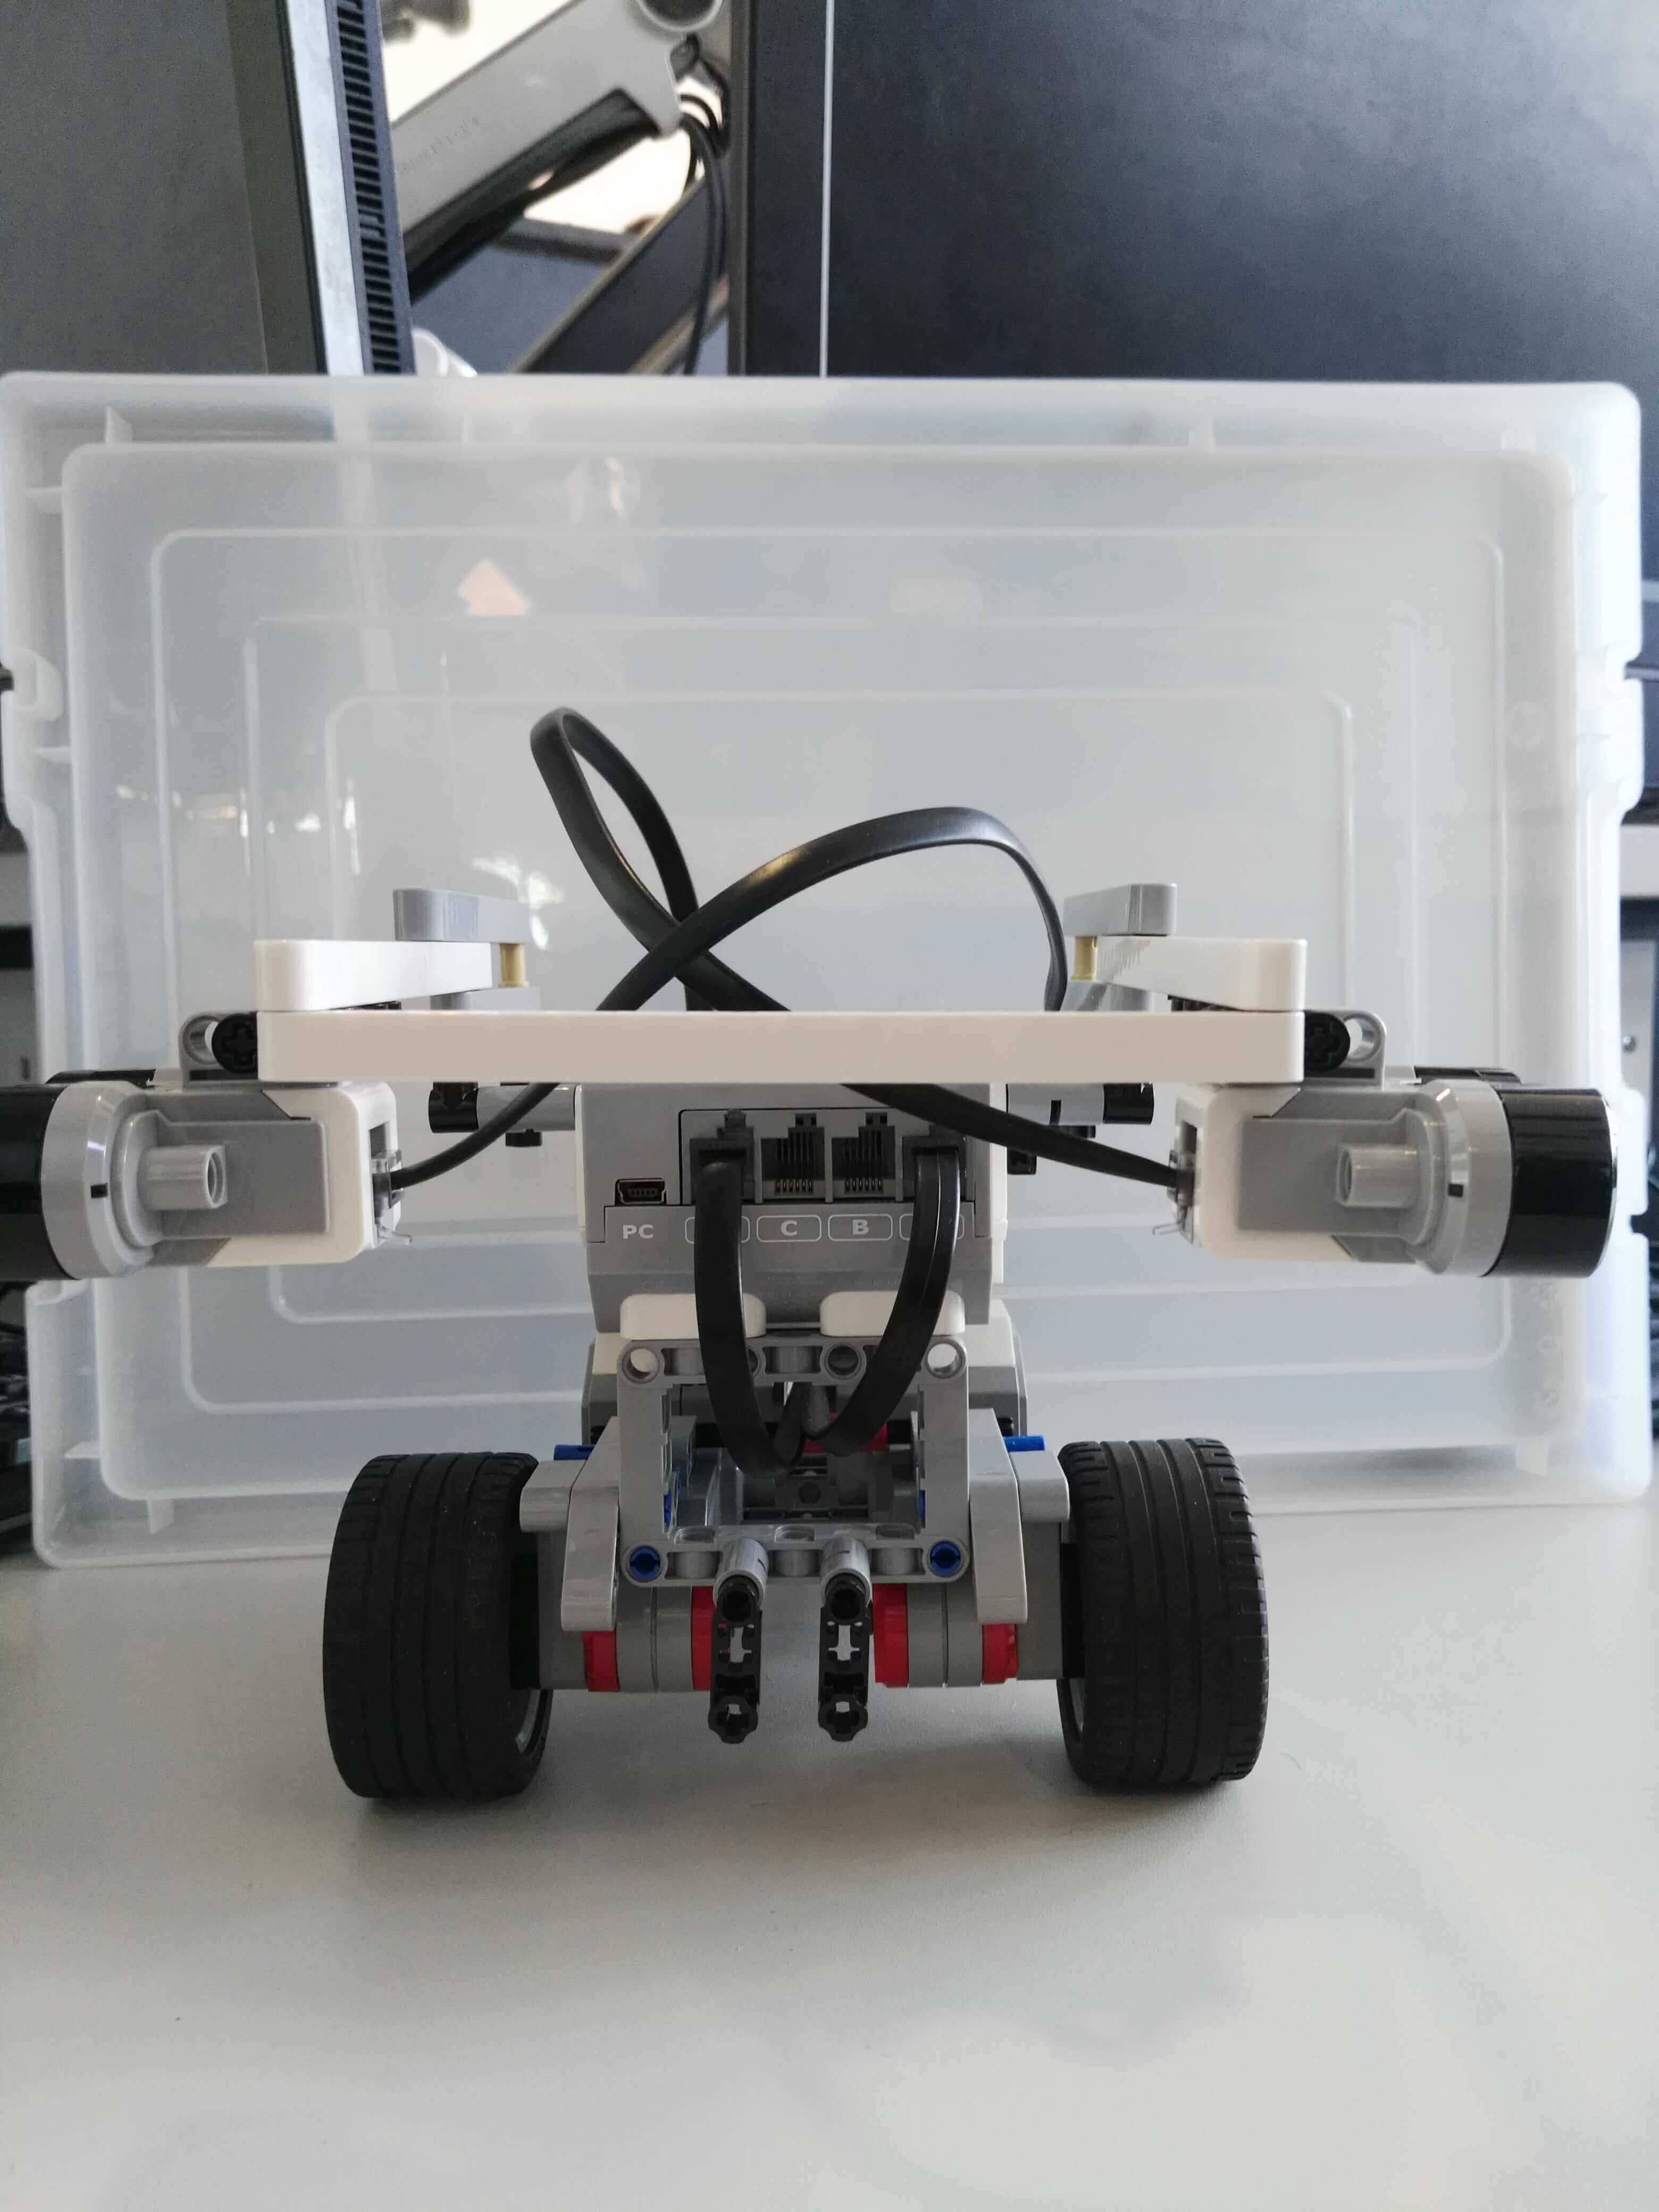
\includegraphics[width=4.5cm]{horizontal3.jpg}
\textbf{Figure 6: Horizontal sensor configuration (first prototype)}
\end{center}
\textbf{Figure 6} showed our first prototype, which is a horizontal positioned sensors in left and
right direction. This prototype is very good at following a straight line but it is not capable of
making a turn effectively. \\

\begin{center}
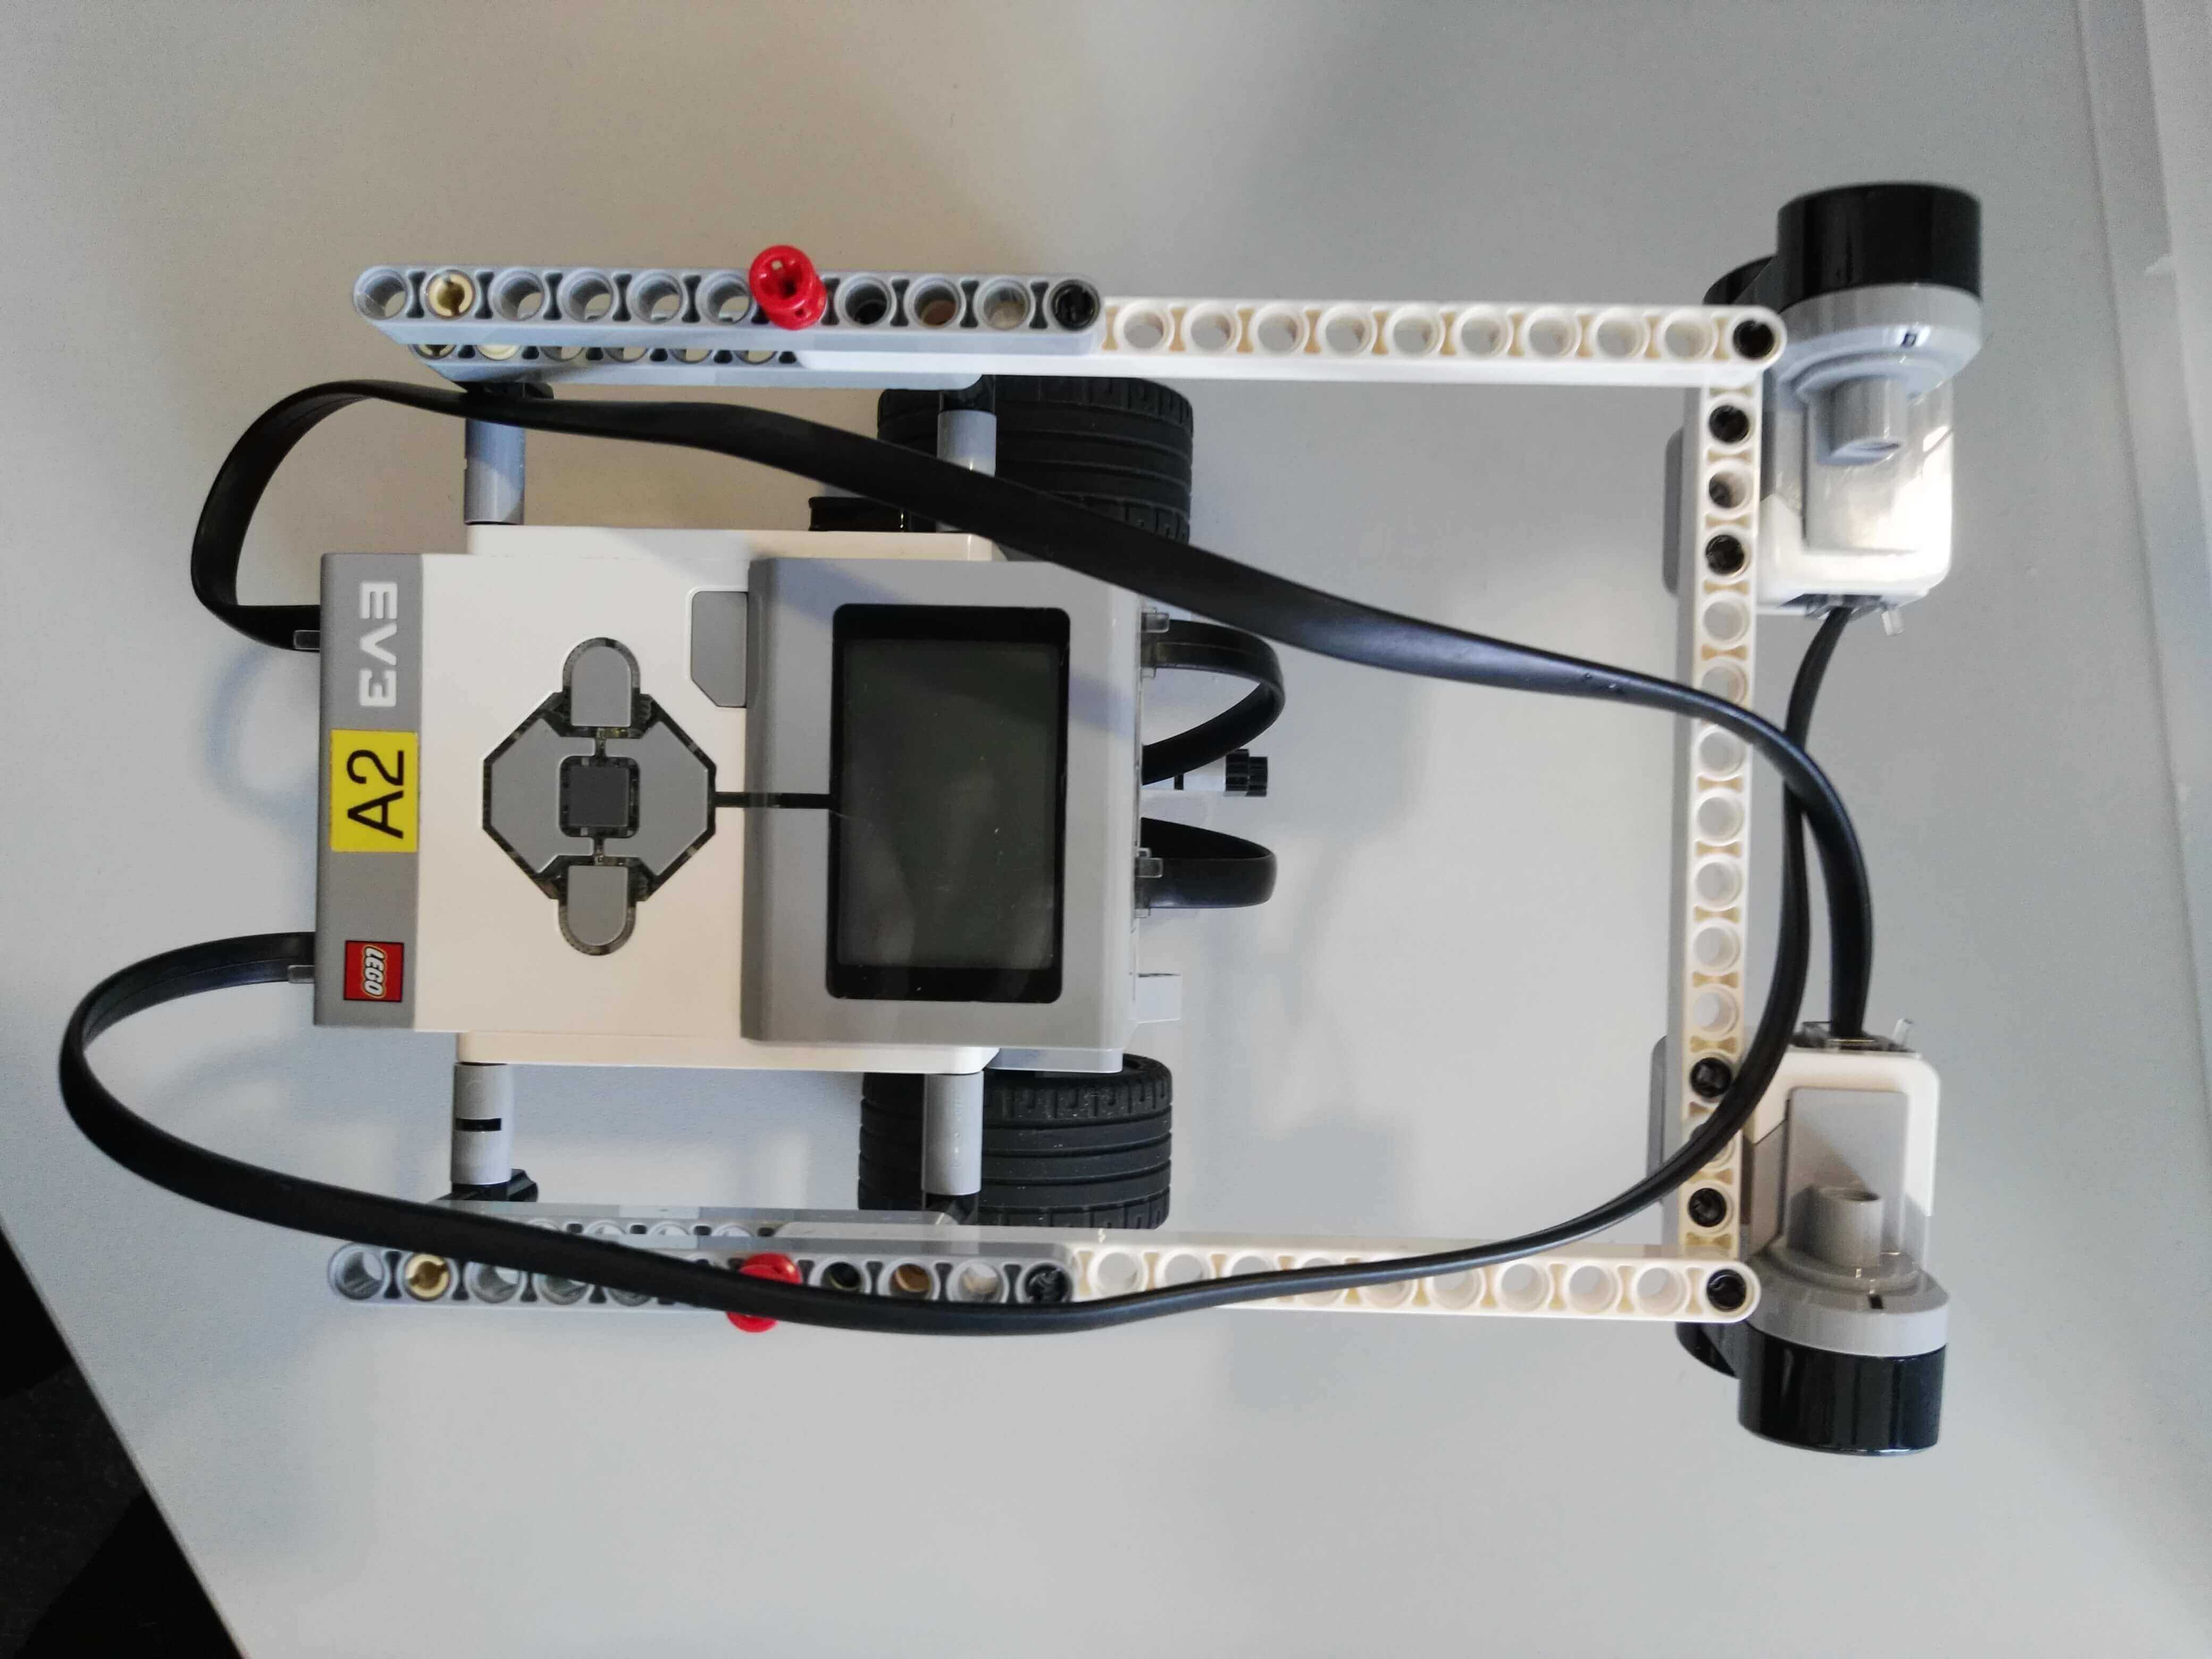
\includegraphics[angle=90, width=4.5cm]{vertical1.jpg}
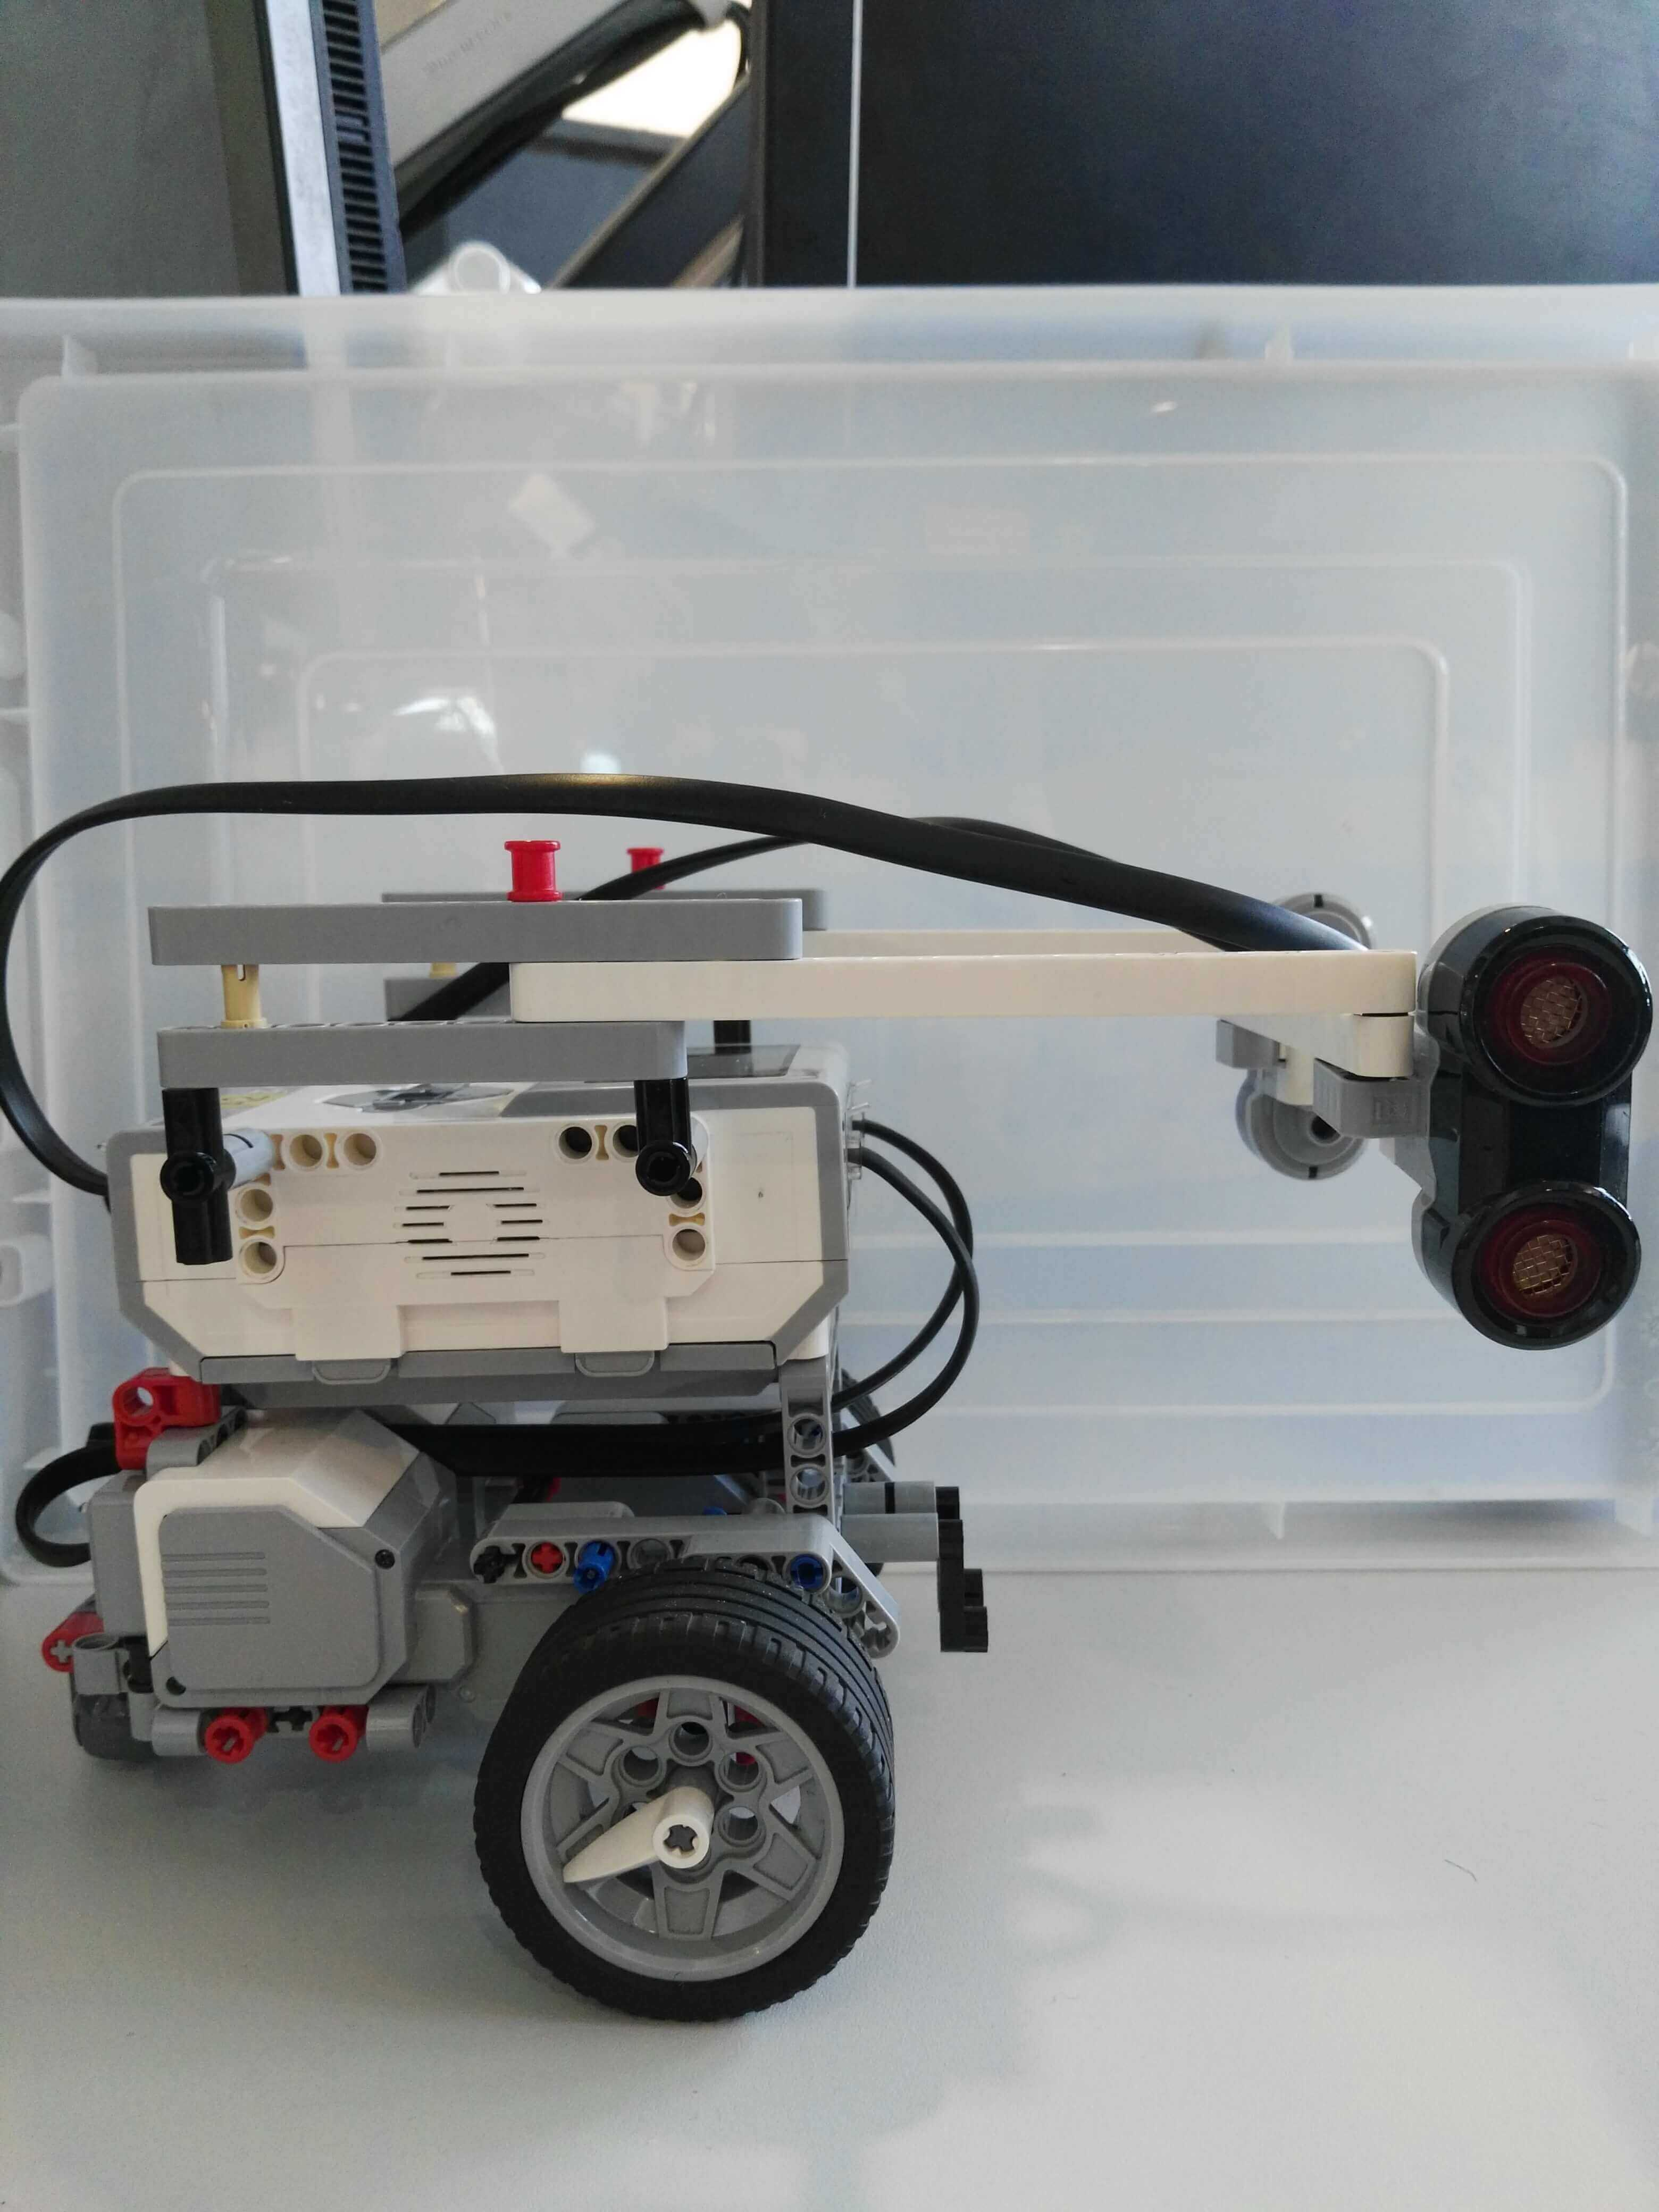
\includegraphics[width=4.5cm]{vertical2.jpg}
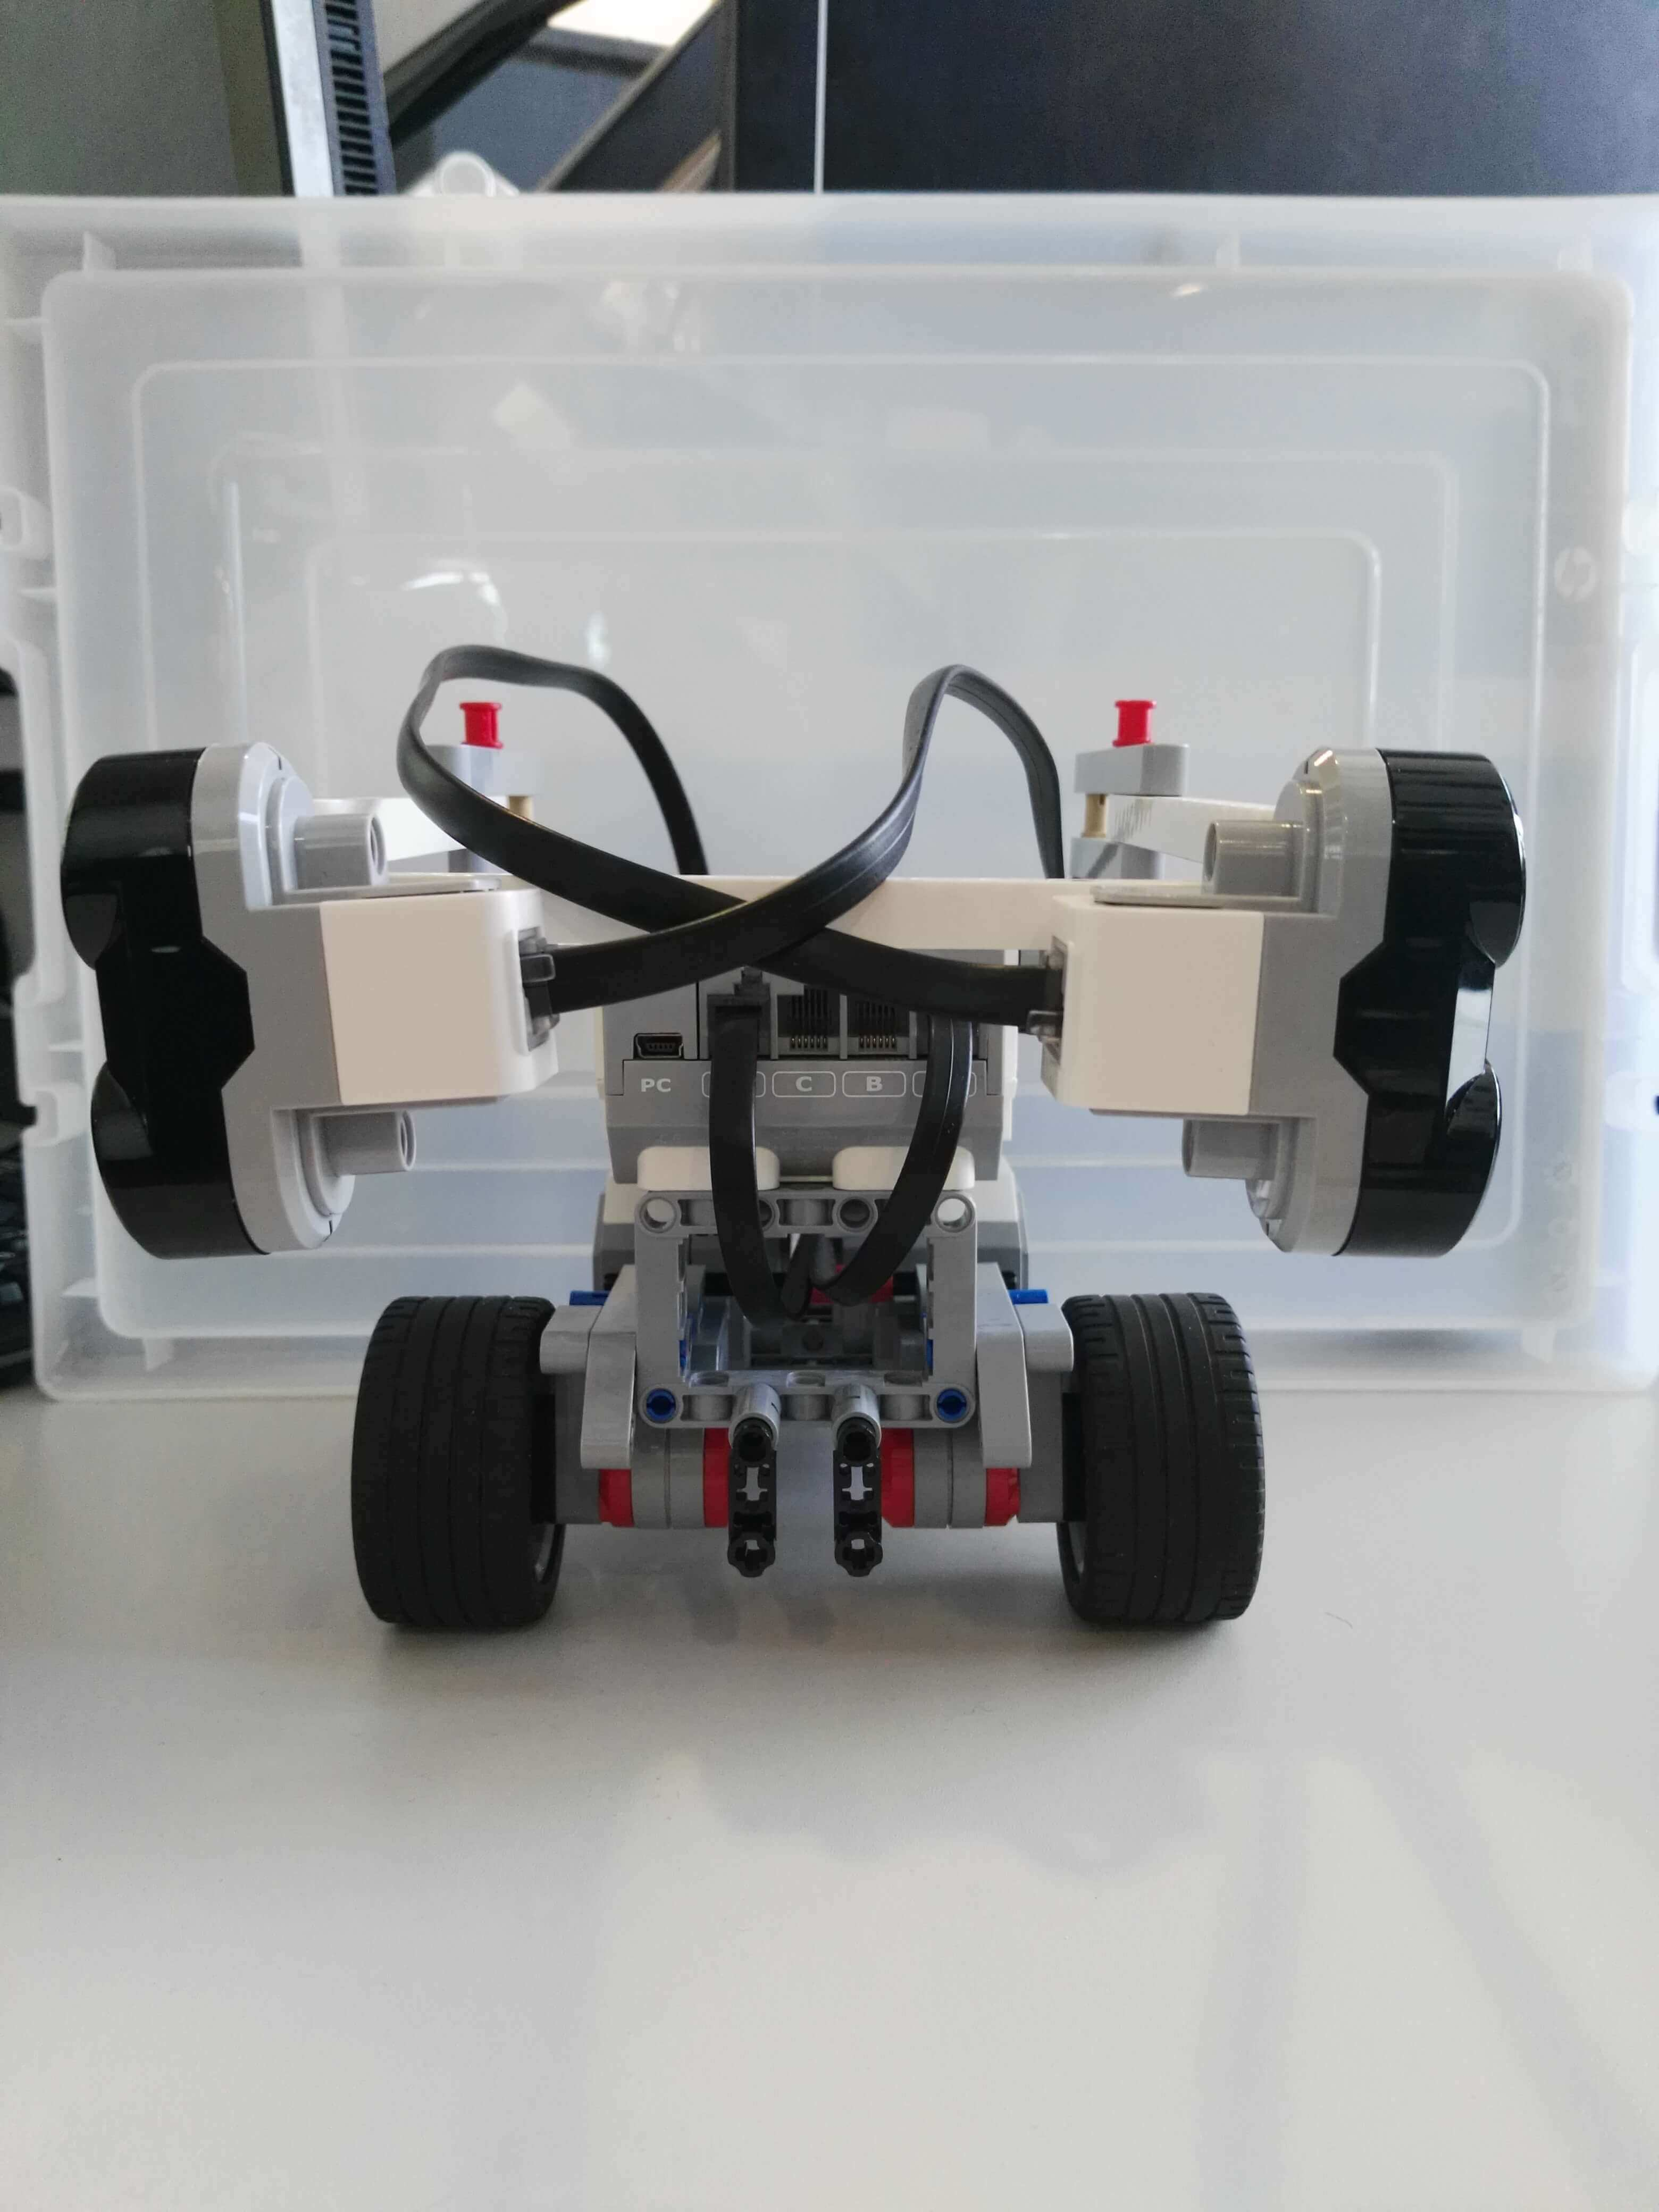
\includegraphics[width=4.5cm]{vertical3.jpg}
\textbf{Figure 7: Vertical sensor configuration (second prototype)}
\end{center}
\textbf{Figure 7} showed our second prototype, which is similar to the first prototype, but the
sensors are positioned vertically. The second prototype has a more restricted horizontal viewing
angle compared to the first prototype. According to our experimentation, the second prototype showed
no noticeable improvement in the maze.
\end{mdframed}
\vspace*{\baselineskip}

{\bfseries Question \myq:}  \emph{What was your robot's final physical configuration (include a
photo)?} (Worth up to 5 marks)\\
\begin{mdframed}
\begin{center}
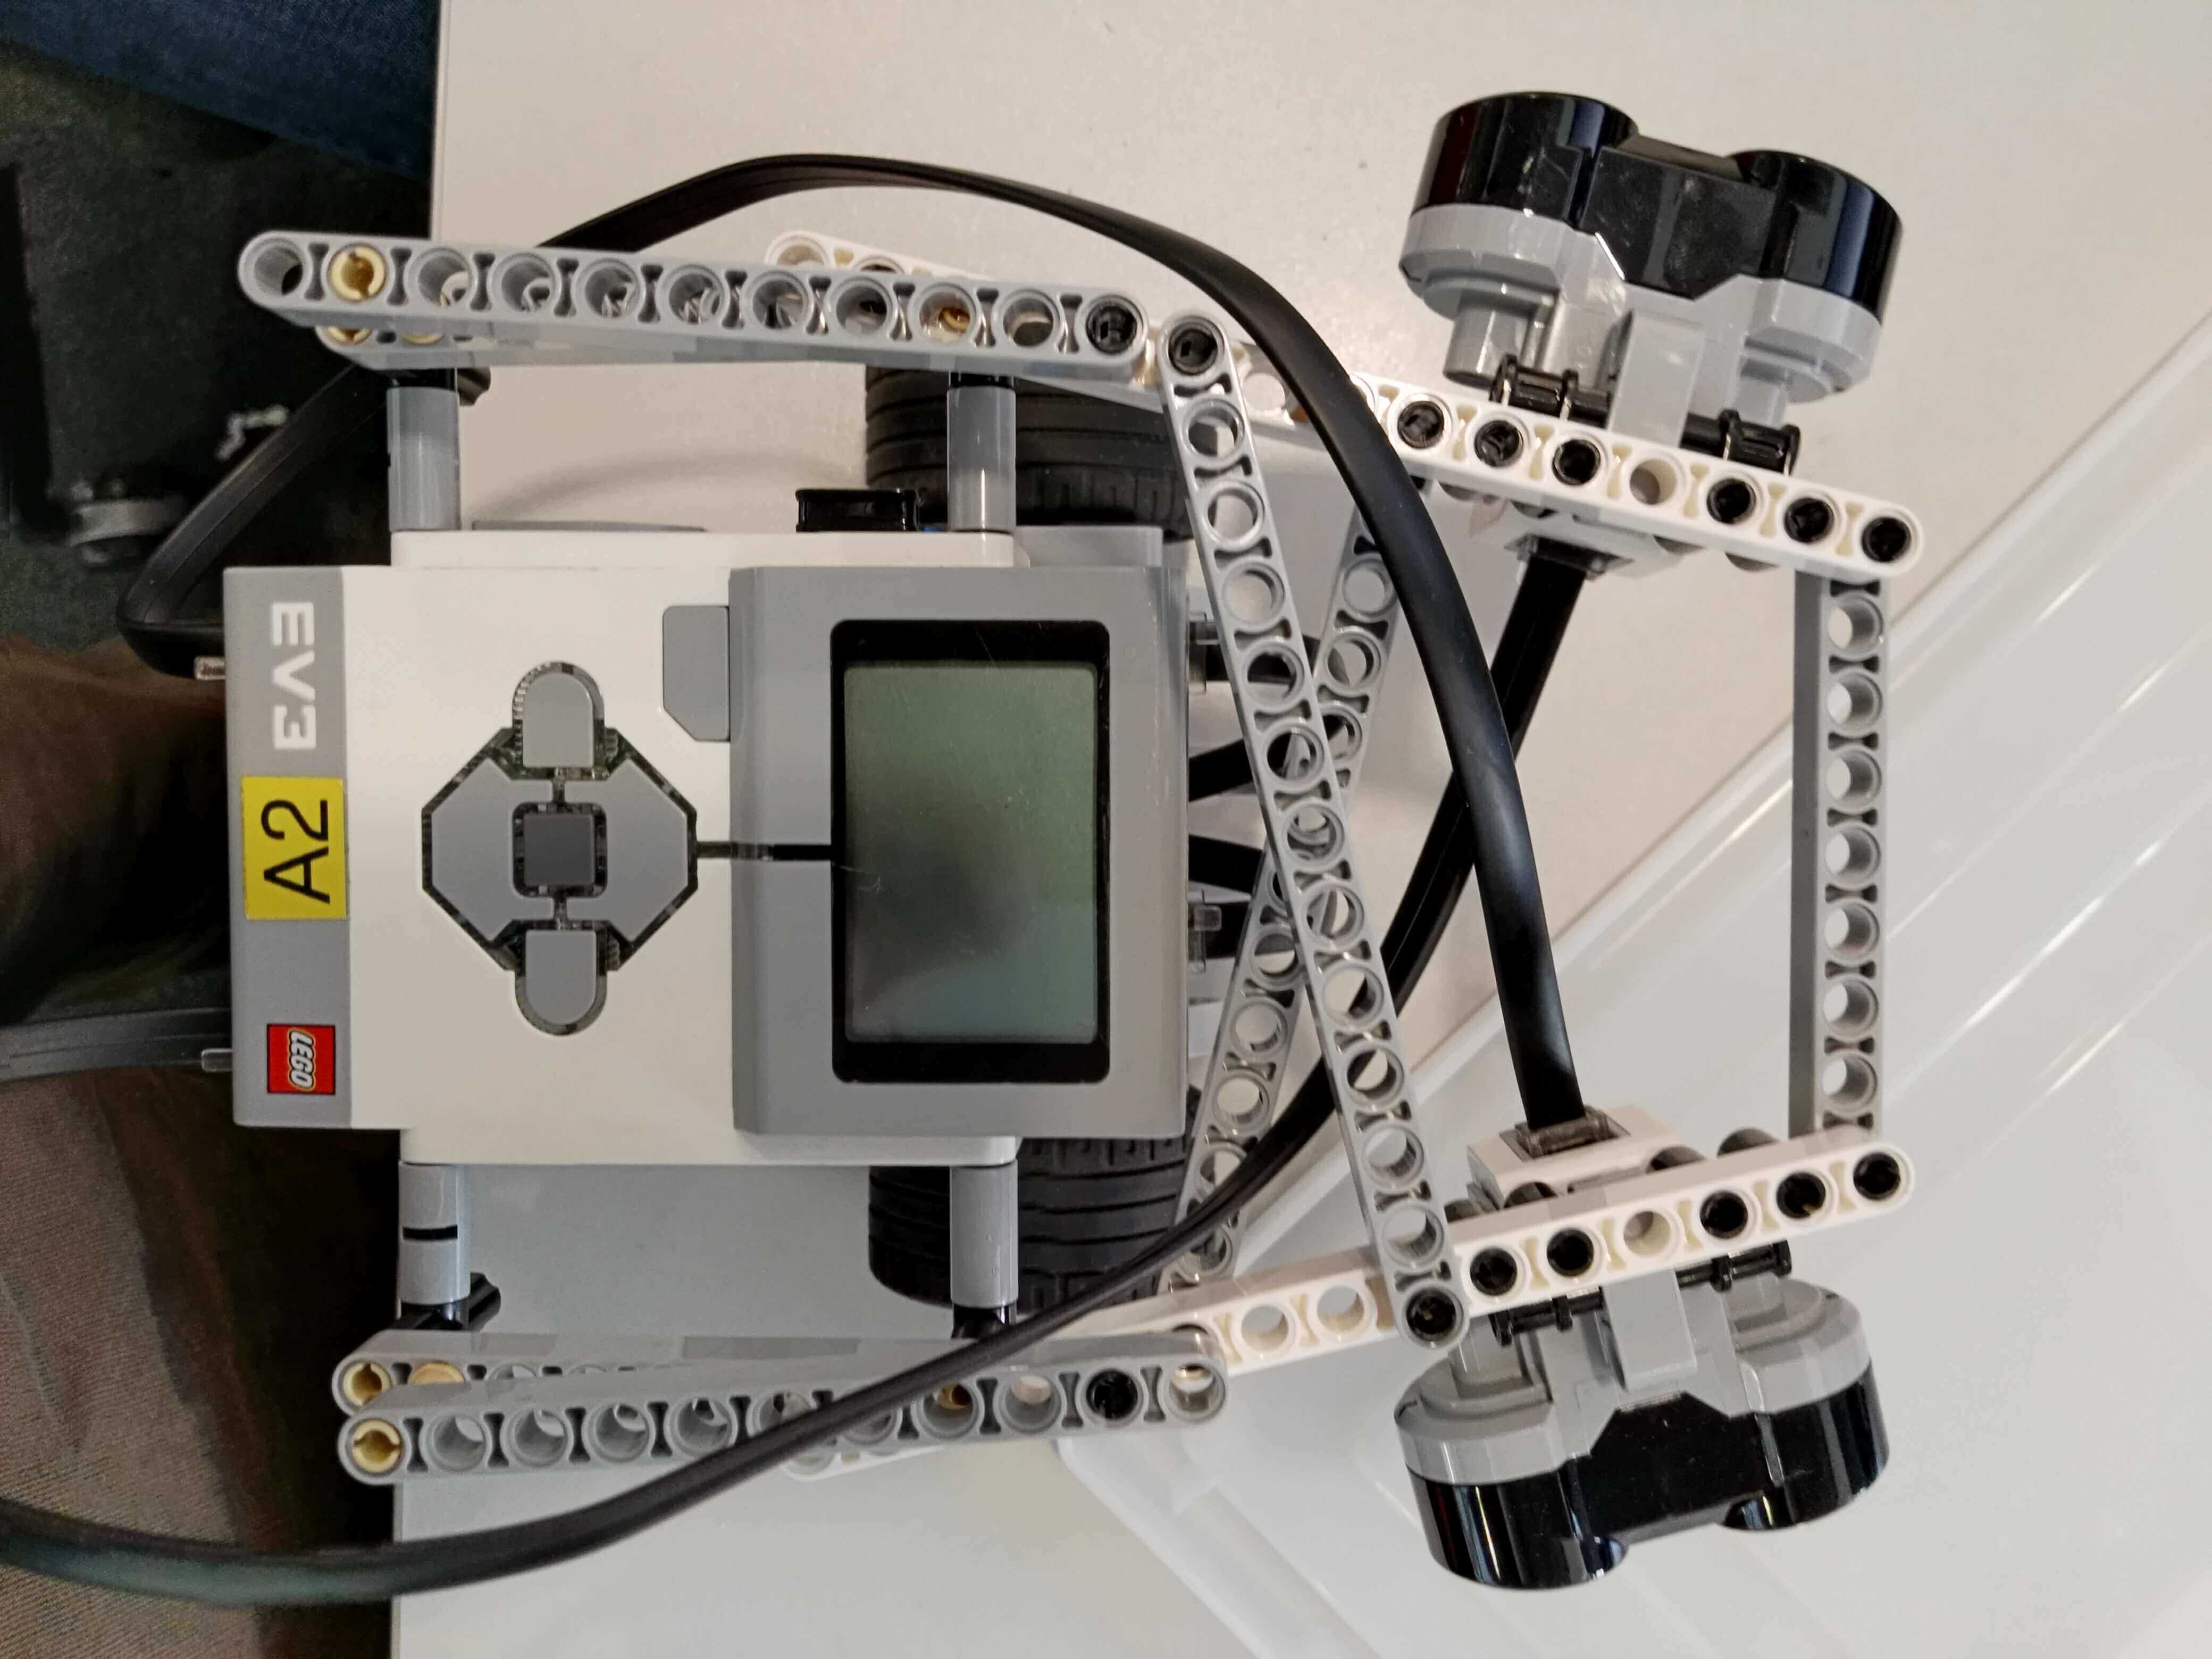
\includegraphics[angle=90, width=4.5cm]{tilt1.jpg}
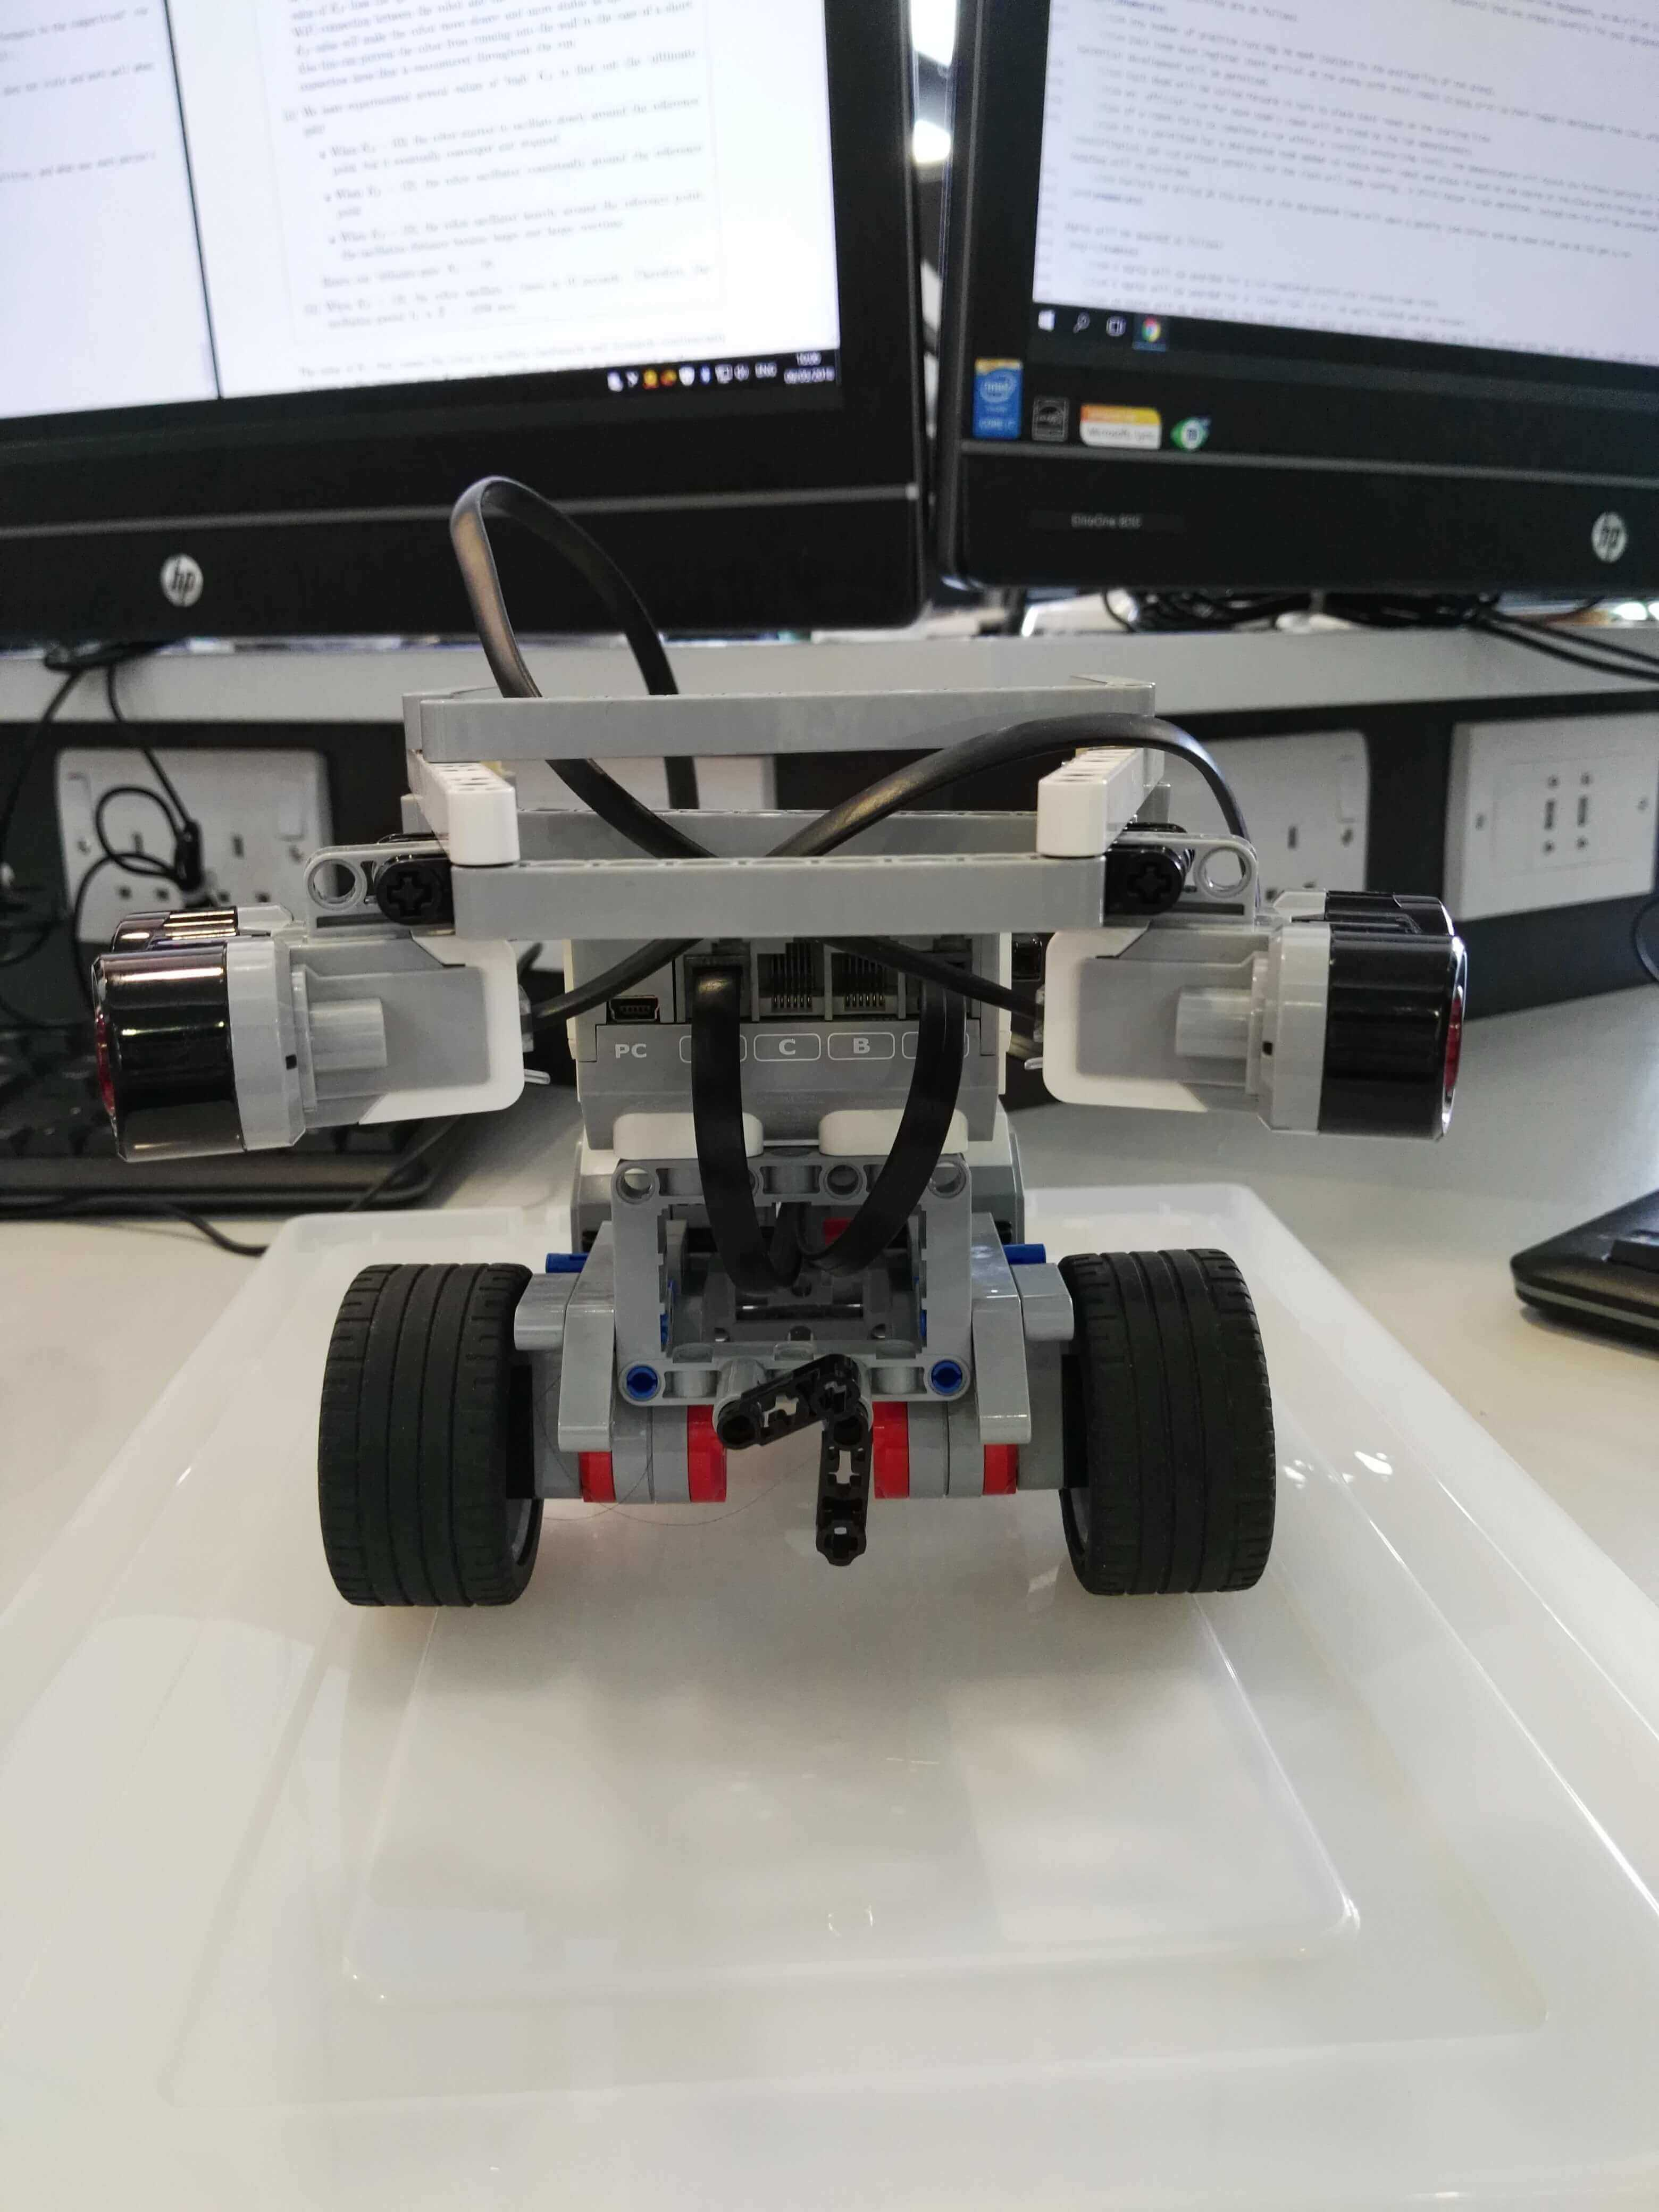
\includegraphics[width=4.5cm]{tilt2.jpg}
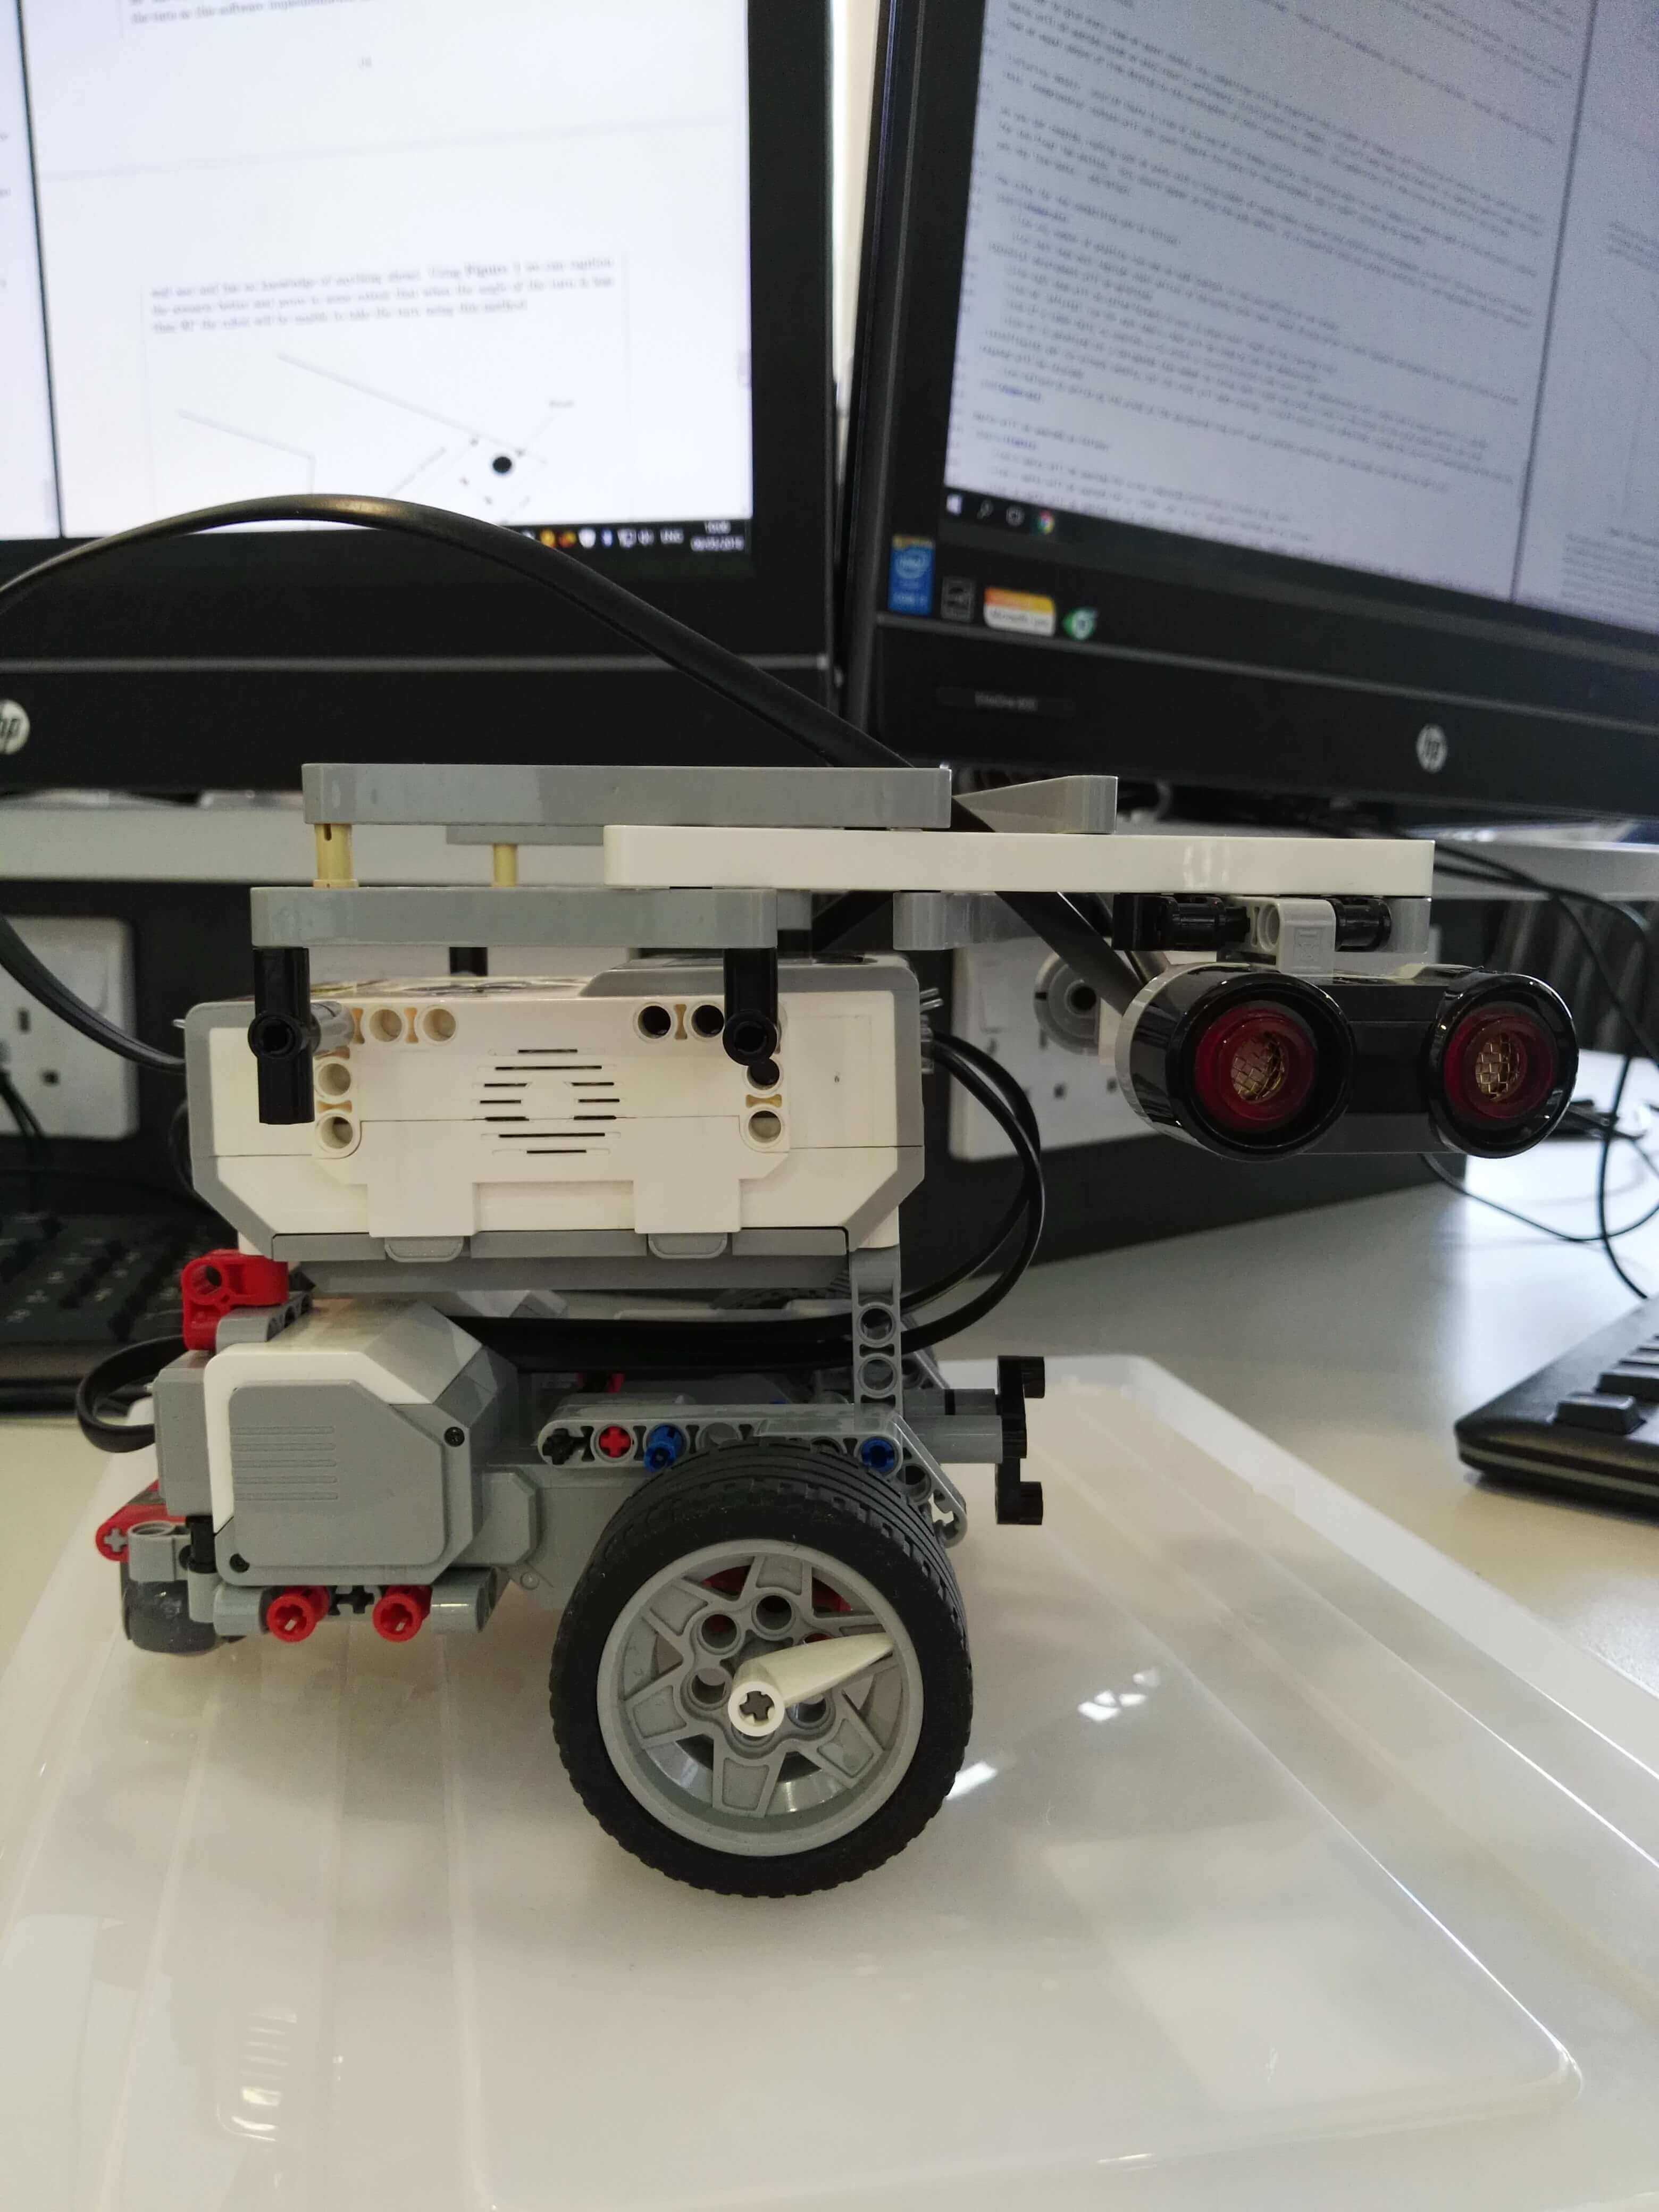
\includegraphics[width=4.5cm]{tilt3.jpg}
\textbf{Figure 8: Final configuration of robot}
\end{center}
The sensors were placed as wide apart as the left and right wheel of the robot, to ensure the most
accurate reading of the walls without making the robot a larger object to manoeuvre. Also as shown
in \textbf{Figure 8}, the sensors were aligned horizontally and not vertically. This was to maximise
the cone of vision of the sensors, as they are more effective in this orientation, and to avoid
accidentally sensing over the walls.

As shown below the angle of the sensors was set slightly forwards, to give it a greater viewing
range, and at the same time allowing it to pick up on the positions of the upcoming walls more
accurately. They were also placed below the supporting horizontal bars to ensure that they did not
accidentally see over the walls.

Crossbars were added in order to give more stability  to the sensors on the robot, as well as extra
bracing horizontal bars to prevent the sensors making it too front heavy
\end{mdframed}
\vspace*{\baselineskip}

{\bfseries Question \myq:}  \emph{Are there any points you wish to make about your robot's
performance in the competition?  For example, if you had had more time, what might you have done
differently?} (Worth up to 5 marks)\\
\begin{mdframed}
During the competition, our robot hit the wall once and had to be rescued, but this was curiously
during the first straight. Due to the fact that it then went to complete all of the rest of the
track perfectly, including the challenging corners, we have to surmise that this was not the fault
of the robot itself. We believe that it may be down to the walls of the maze being comprised of
slats of wood, joined together with hinges, and that the sensor may have seen through one of the
gaps, causing the robot to continue on its path towards the opposite wall instead of correcting.

One of our robot's weaknesses is taking wide turns in the maze. The position of the sensors does not
scale well, so our robot always took the outside line around a wide turn. Changing this so it
follows the inner wall of the turn would reduce the time taken by our robot to make the turn hence
improving our overall competition time.

Another weakness is that our robot will always try to maintain a equal distance between the left
wall and right wall. This causes the robot to keep turning left and turning right even though it is
following a straight wall, resulting in a slower completion time compared to those which followed
the wall smoothly.

Given more time, we would also have experimented more with the values in-putted into our PID
controller, to find values of $K_P$, $K_I$ and $K_D$ that would best improve the quality control of
the controller, making it navigate through the maze quicker without colliding with any walls. We
would also implement the robot in a way such that it does not always maintain an equal distance
between the left and right wall, but it only adjusts itself when it is too close to the wall. This
would have made the robot movement much smoother.
\end{mdframed}
\vspace*{\baselineskip}

Finally, how did you organise your team?  I.e.\ what was each member's role and responsibilities,
and what was each person's contribution as a \%?  Please fill in the Table below:
\begin{center}
	\begin{tabular}{ | c | p{8cm} | c | } \hline
		 \bf{Team Member} & \bf{Role} & \% \\ \hline
         Catalin Mares & Research, report & 21 \\ \hline
         David Coelho & System design, report & 21 \\ \hline
		Huzaifa Ahmed & Research, report & 16 \\ \hline
        Joseph Slade & Physical design, report & 21 \\ \hline
		Zer Jun Eng & Coding, research, report & 21 \\ \hline

	\end{tabular}
\end{center}

\end{document}
